\subsection{NuMI as a Sideband}
MicroBooNE is exposed to an orthogonal, sizable source of neutrinos which can be used as sideband to cross check BNB $\nu_e$ searches: the NuMI beam.  Albeit the energy of the protons generating the NuMI beam is much higher (120 GeV protons from the Main Injector compared to the usual 8 GeV of the Booster),  neutrinos from NuMI cover an energy range similar to the neutrinos from BNB, because of the highly off-axis nature of the NuMI beam at MicroBooNE. Additionally, the electron $\nu_e$ and $\bar\nu_e$ content of the beam is about an order of magnitude higher in NuMI compared to the intrinsic $\nu_e$ BNB prediction, and  oscillation effects in NuMI are predicted to be small -- as well as extremely difficult to disentangle from the flux predictions for the intrinsic electron neutrinos. These characteristics make NuMI data ideal to benchmark the analysis in a enriched electron neutrino environment on the full energy spectrum.

\subsubsection{Overview of NuMI data set}
The availability of NuMI data has been limited. Thus, the results presented in this section are obtained only with a Run 1 sample of 8.885e19 POT on beam and $\sim$4M EXT triggers (both corresponding to about half of the  Run 1 collected sample), as well as simulated $\nu$ overlay and dirt samples corresponding to 2.071e21 POT  and 1.421e21 POT, respectively. The result presented only show statistical uncertainty, not considering cross section or flux systematics. Details on the NuMI beam  flux predictions can be found in Ref.~\cite{bib:NuMIFlux}. We follow the current best practices for NuMI POT normalization in MCC9, which entail a reduction of the NuMI EXT trigger by 2\% (to account for neutrino trigger occupancy) and a reduction of the dirt by 65\% (constraint using the event flash timing); more details on the NuMI POT normalization can be found in \cite{bib:NuMINorm}. 


\subsubsection{NuMI 
\npsel Sideband}
Figure~\ref{fig:NuMI_1eNp_reco_e} shows the reconstructed energy spectrum for \npsel after the final \npsel selection using the currently available 8.885e19  POT from Run 1 NuMI data. As desired in absence of oscillations, data-MC agree on the full energy spectrum including at low energies, providing a solid validation for this selection.

\begin{figure}[H]
    \begin{center}
    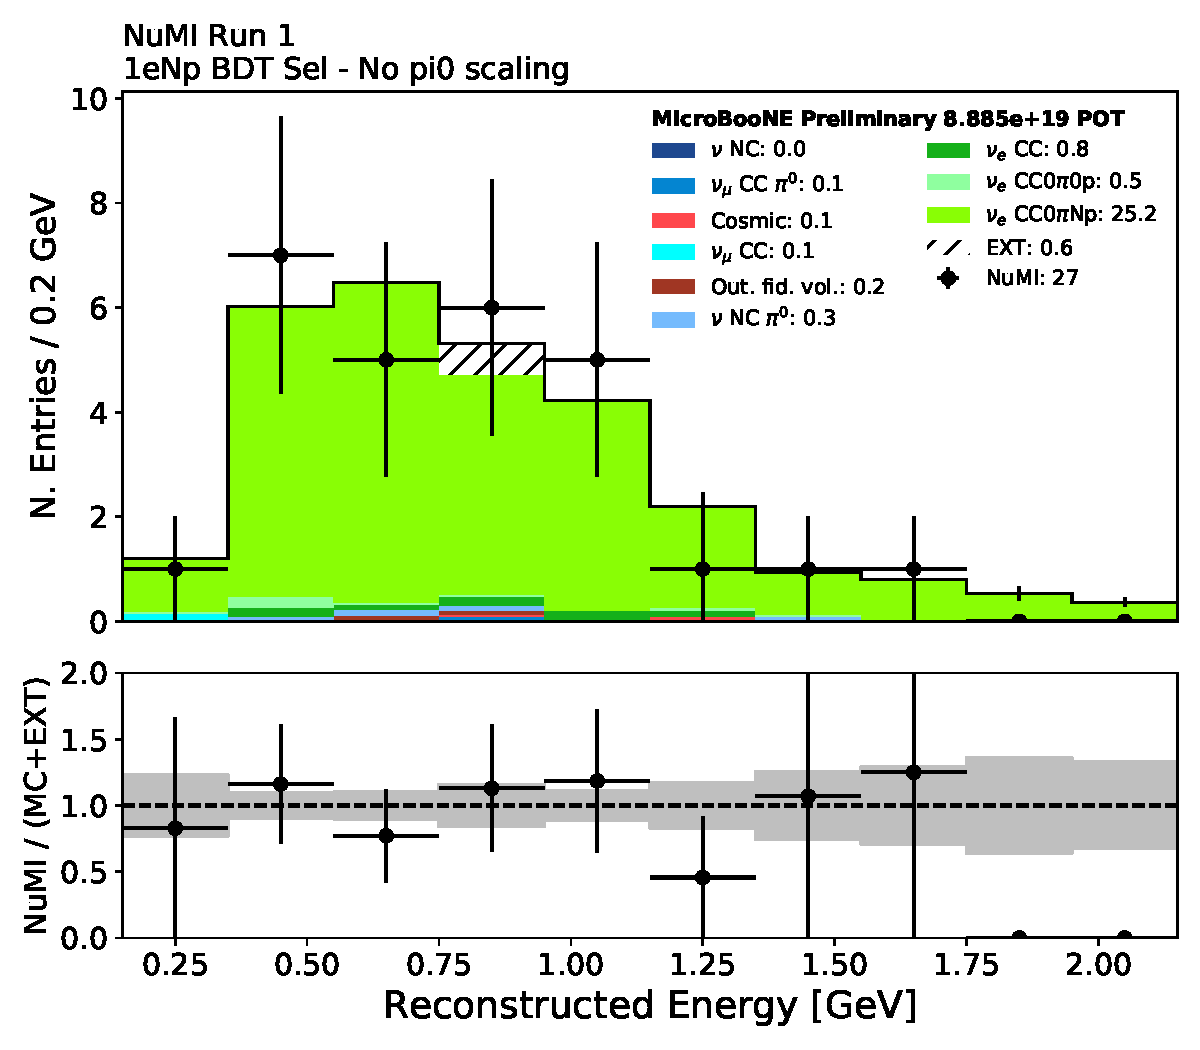
\includegraphics[width=0.5\textwidth]{Sidebands/Figures/NuMI/1eNp/BDTSel/reco_e.pdf}
    \caption{Reconstructed neutrino energy after \npsel BDT selection on NuMI data.}
    \label{fig:NuMI_1eNp_reco_e}
    \end{center}
\end{figure}


Additional cross checks on the BDT input variables at the loose selection stage on the NuMI dataset have been performed, finding good agreement across most distributions. The complete Data-MC comparison can be found in \cref{app:sideband:1eNpNuMI}. Figures~\ref{fig:NuMI_1eNp_0} show some examples of BDT input variables for key distributions such as track PID and shower dE/dx in this $\nu_e$ rich sample. Figures~\ref{fig:NuMI_1eNp_7} show the BDT response from the \npsel NuMI sideband, again presenting good data-MC agreement.

\begin{figure}[H]
    \centering
    \begin{subfigure}{0.3\textwidth}
    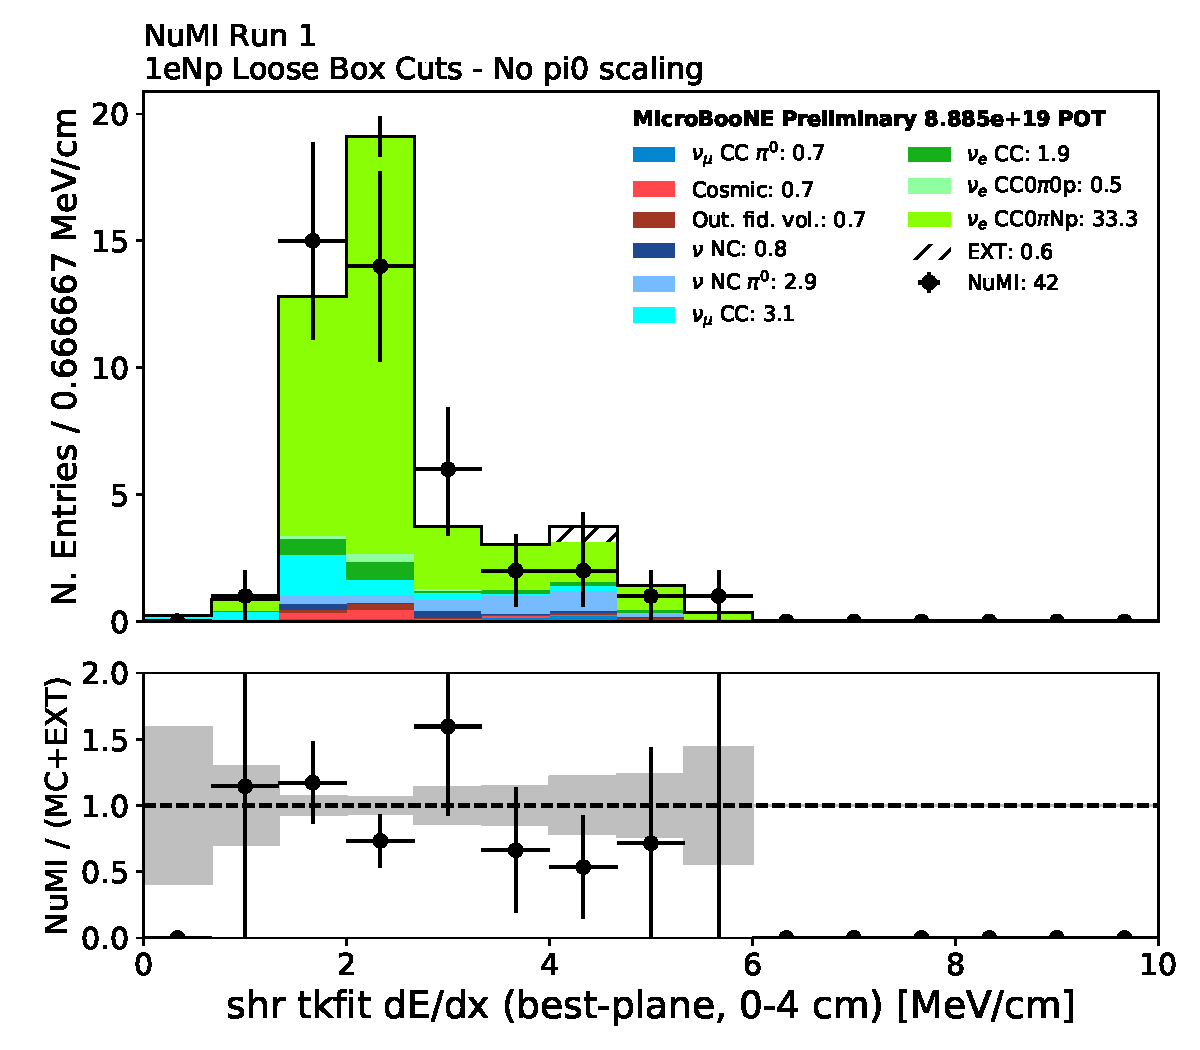
\includegraphics[width=1.0\textwidth]{Sidebands/Figures/NuMI/1eNp/shr_tkfit_dedx_max.pdf}
    \caption{shr\_tkfit\_dedx\_max}
    \end{subfigure}
    \begin{subfigure}{0.3\textwidth}
    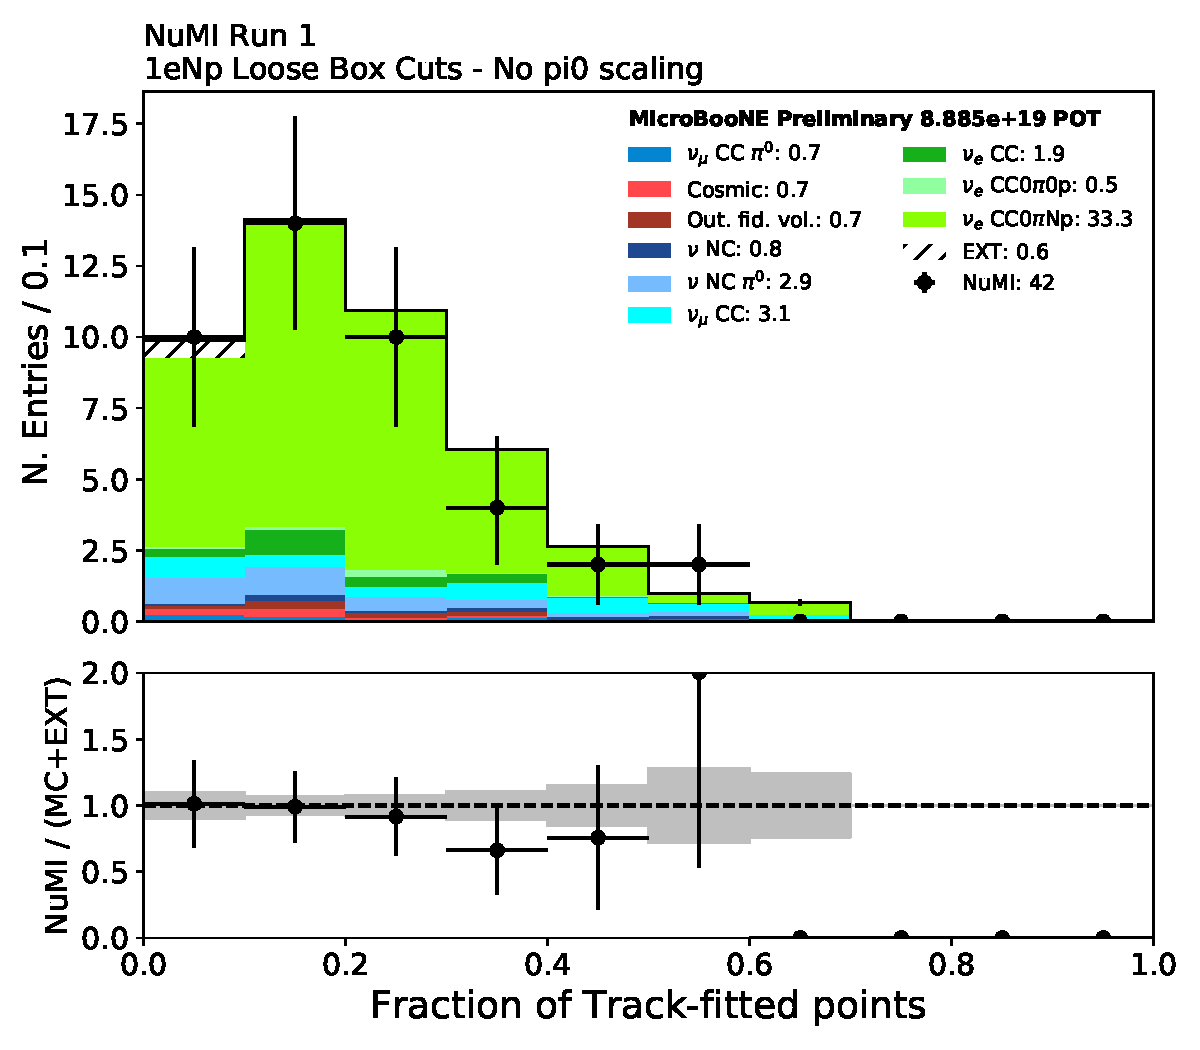
\includegraphics[width=1.0\textwidth]{Sidebands/Figures/NuMI/1eNp/trkfit.pdf}
    \caption{trkfit}
    \end{subfigure}
    \begin{subfigure}{0.3\textwidth}
    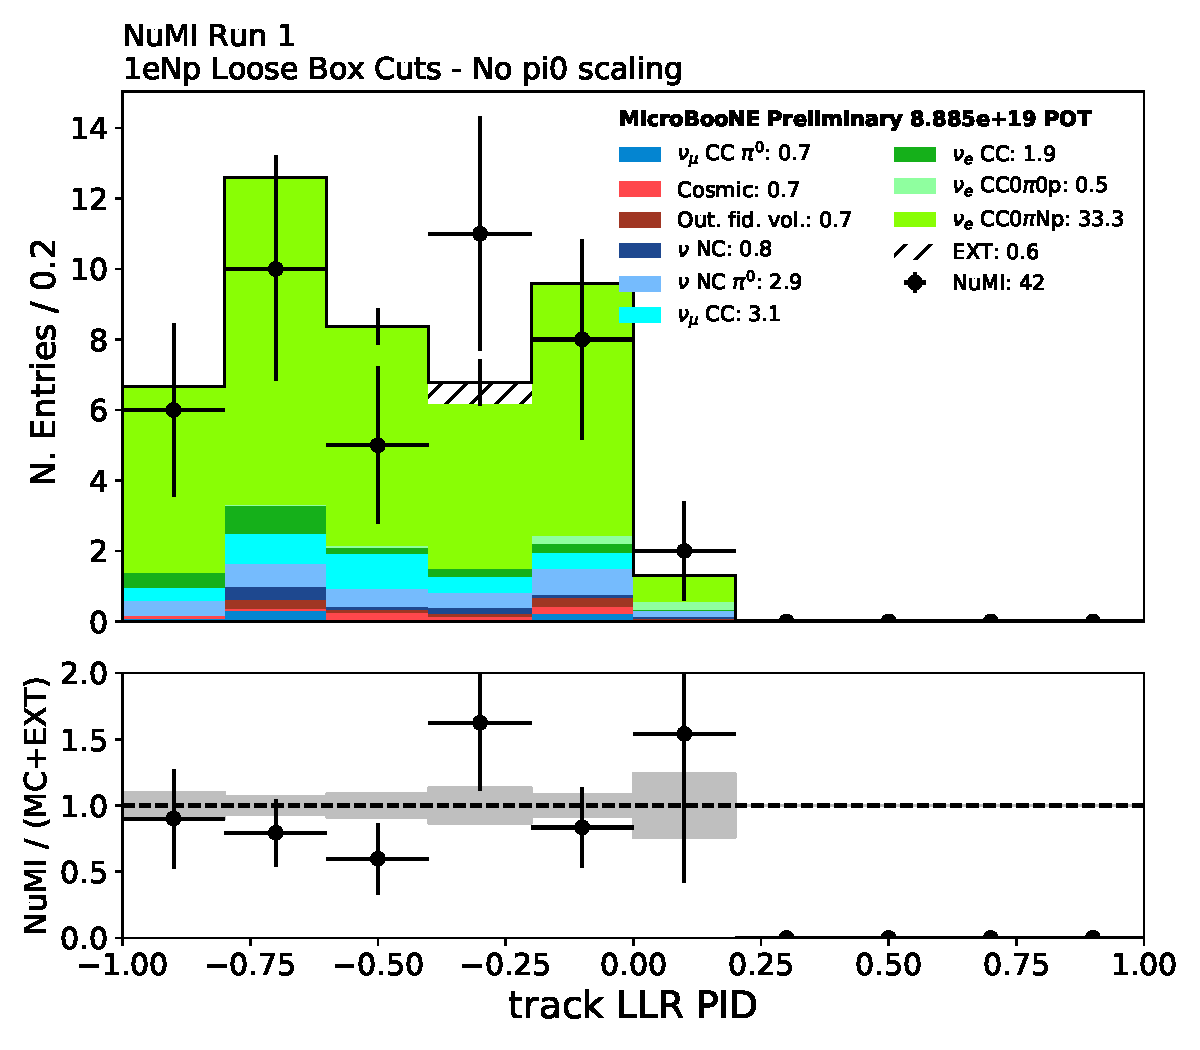
\includegraphics[width=1.0\textwidth]{Sidebands/Figures/NuMI/1eNp/trkpid.pdf}
    \caption{trkpid}
    \end{subfigure}
    \caption{Select BDT input variables after \npsel Loose selection on NuMI data.} 
    \label{fig:NuMI_1eNp_0}
\end{figure}

\begin{comment}
\begin{figure}[H]
    \centering
    \begin{subfigure}{0.3\textwidth}
    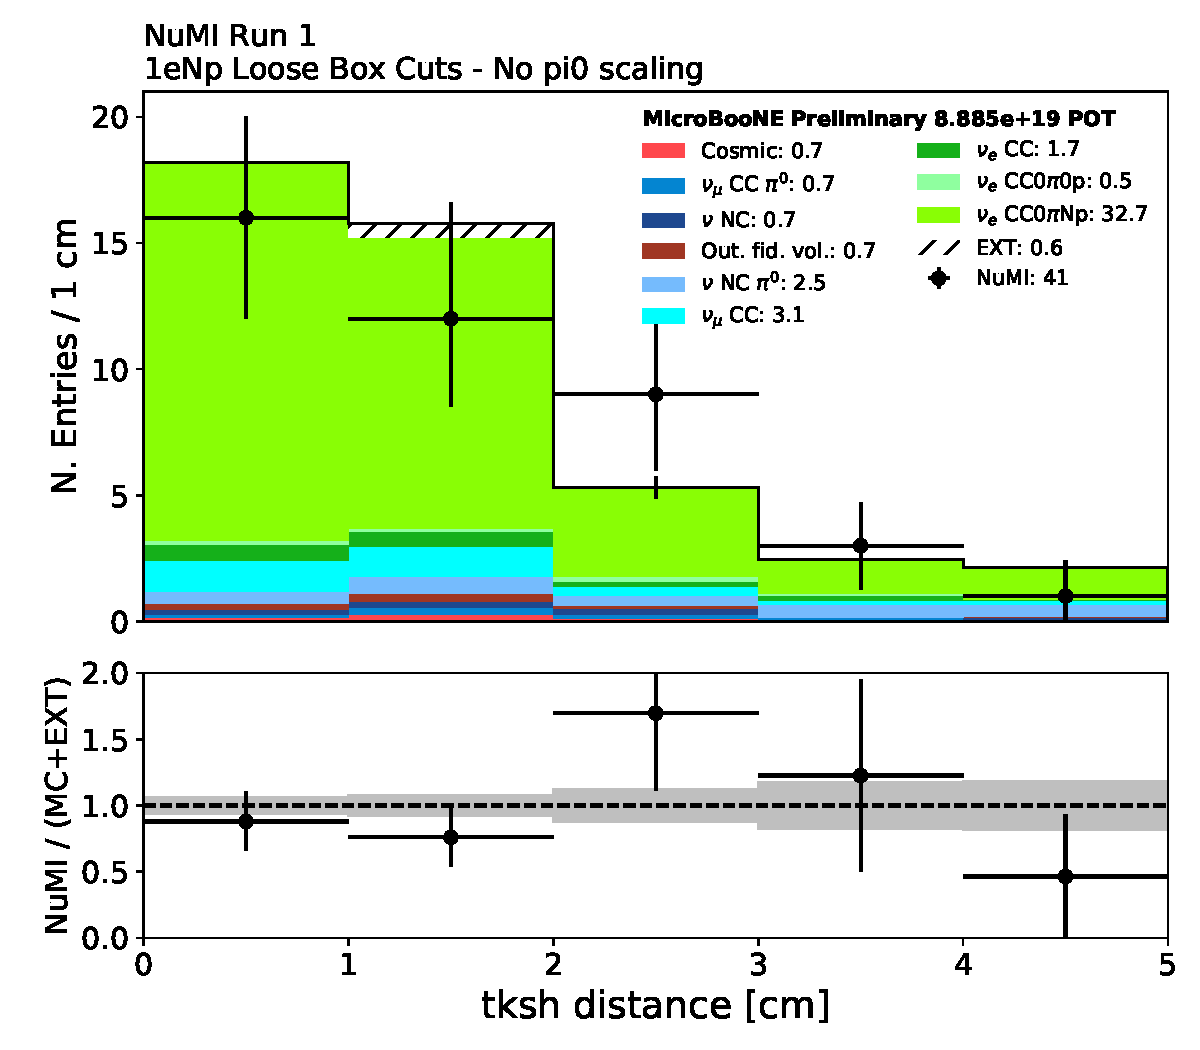
\includegraphics[width=1.0\textwidth]{Sidebands/Figures/NuMI/1eNp/tksh_distance.pdf}
    \caption{tksh\_distance}
    \end{subfigure}
    \begin{subfigure}{0.3\textwidth}
    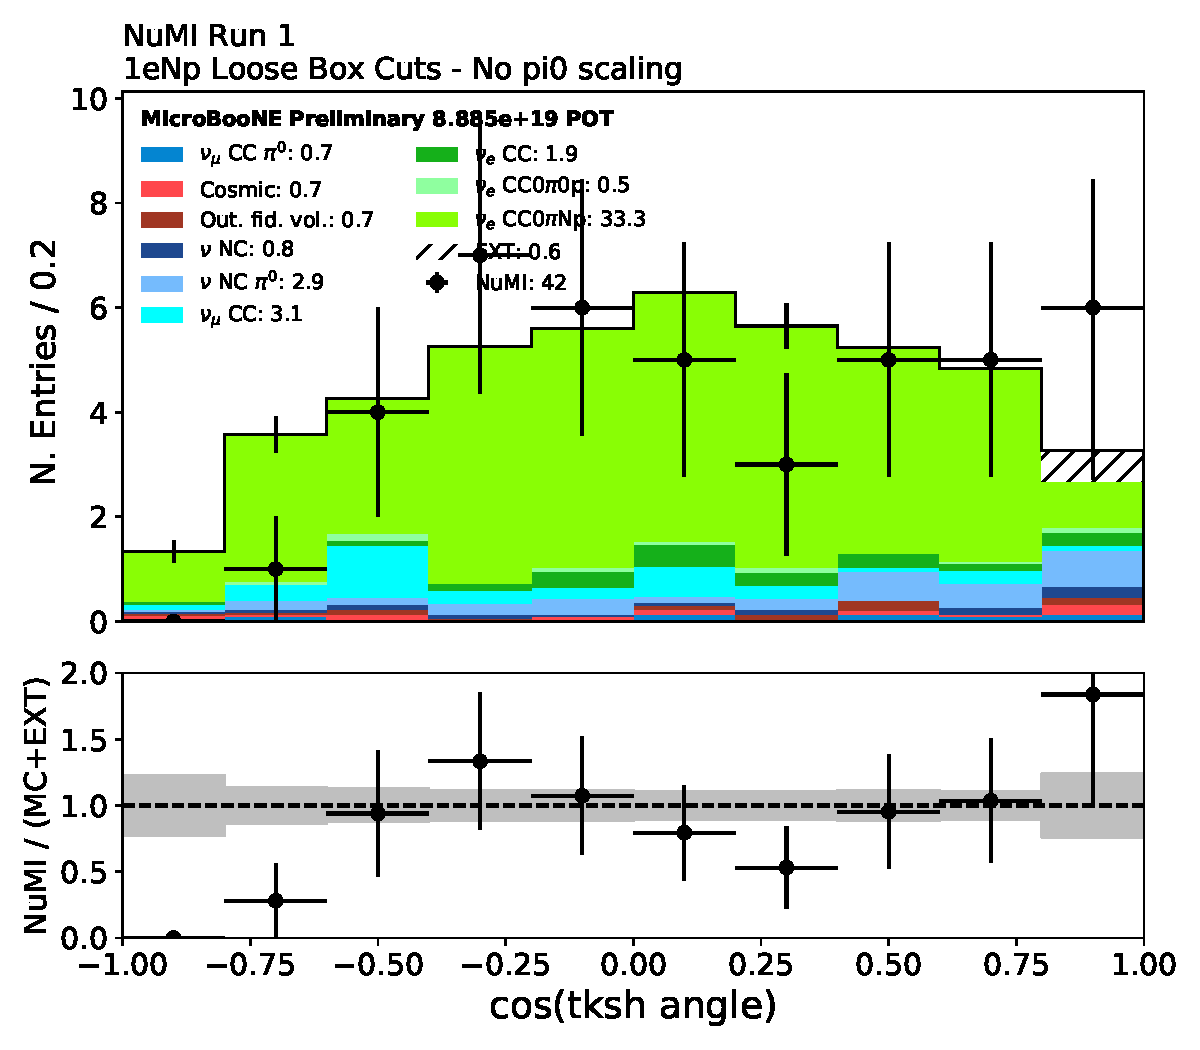
\includegraphics[width=1.0\textwidth]{Sidebands/Figures/NuMI/1eNp/tksh_angle.pdf}
    \caption{tksh\_angle}
    \end{subfigure}
    \begin{subfigure}{0.3\textwidth}
    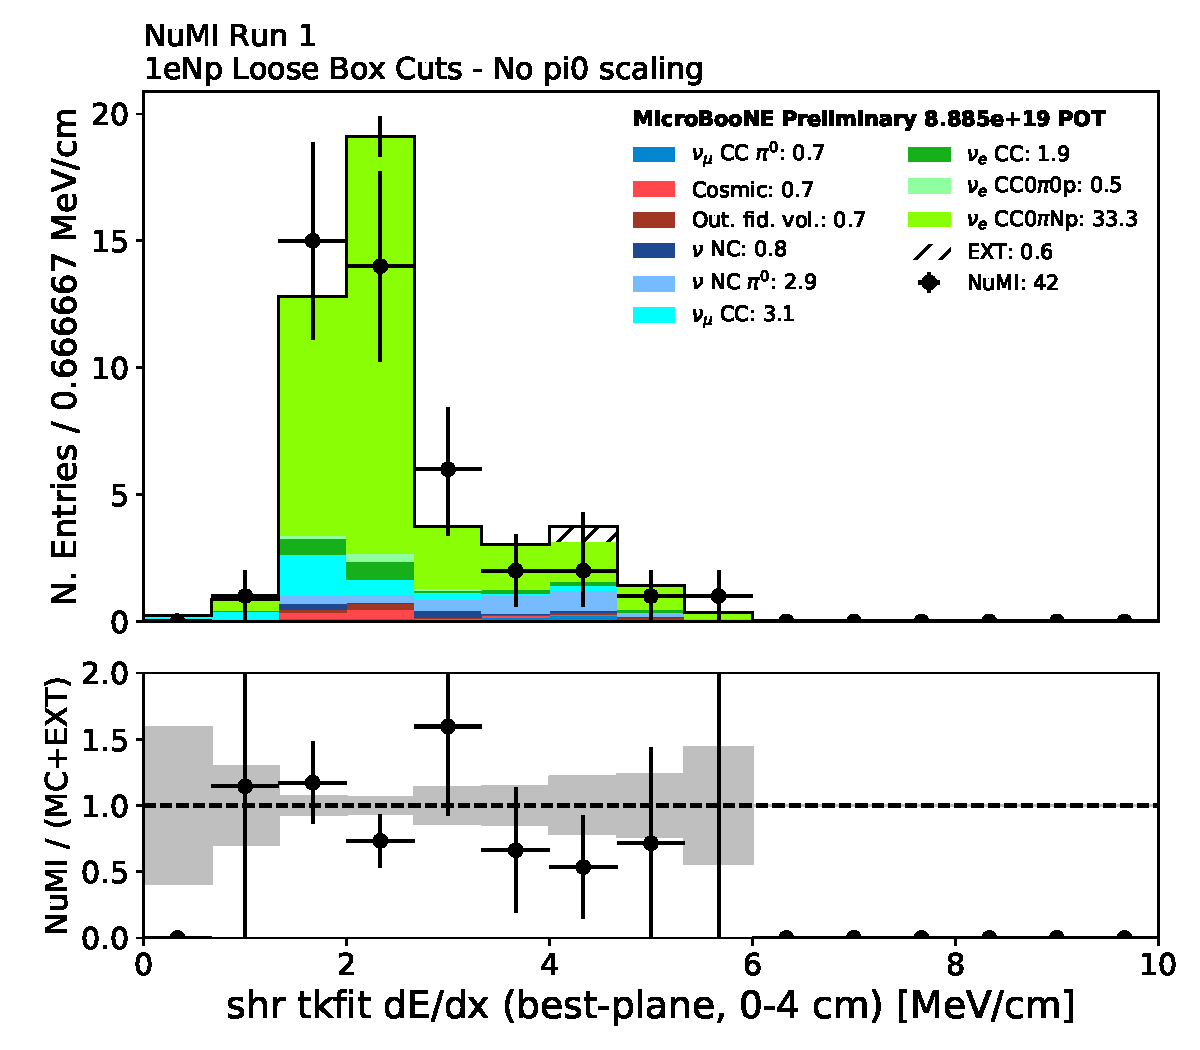
\includegraphics[width=1.0\textwidth]{Sidebands/Figures/NuMI/1eNp/shr_tkfit_dedx_max.pdf}
    \caption{shr\_tkfit\_dedx\_max}
    \end{subfigure}
    \caption{} 
    \label{fig:NuMI_1eNp_1}
\end{figure}

\begin{figure}[H]
    \centering
    \begin{subfigure}{0.3\textwidth}
    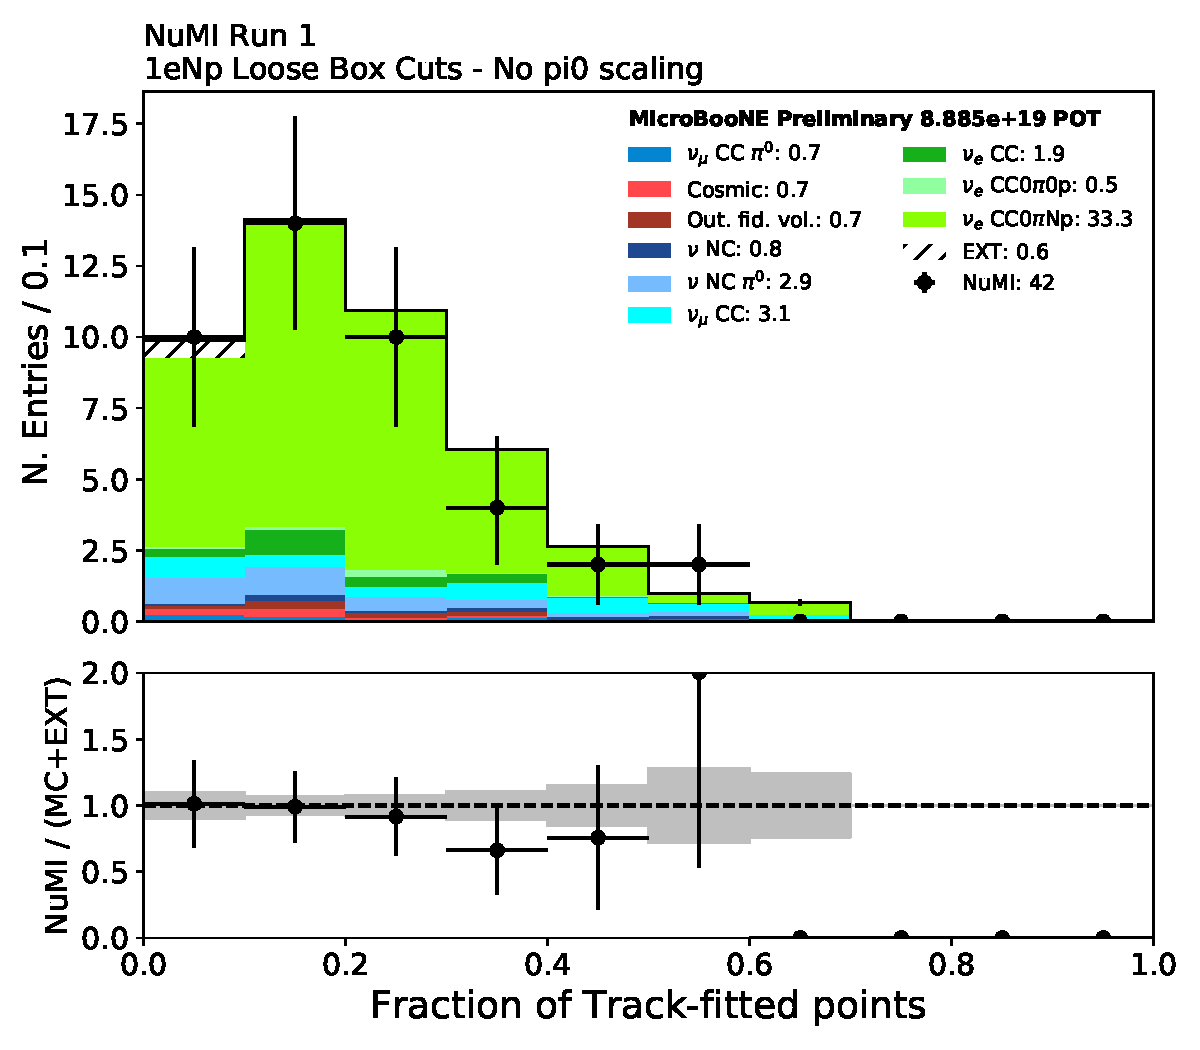
\includegraphics[width=1.0\textwidth]{Sidebands/Figures/NuMI/1eNp/trkfit.pdf}
    \caption{trkfit}
    \end{subfigure}
    \begin{subfigure}{0.3\textwidth}
    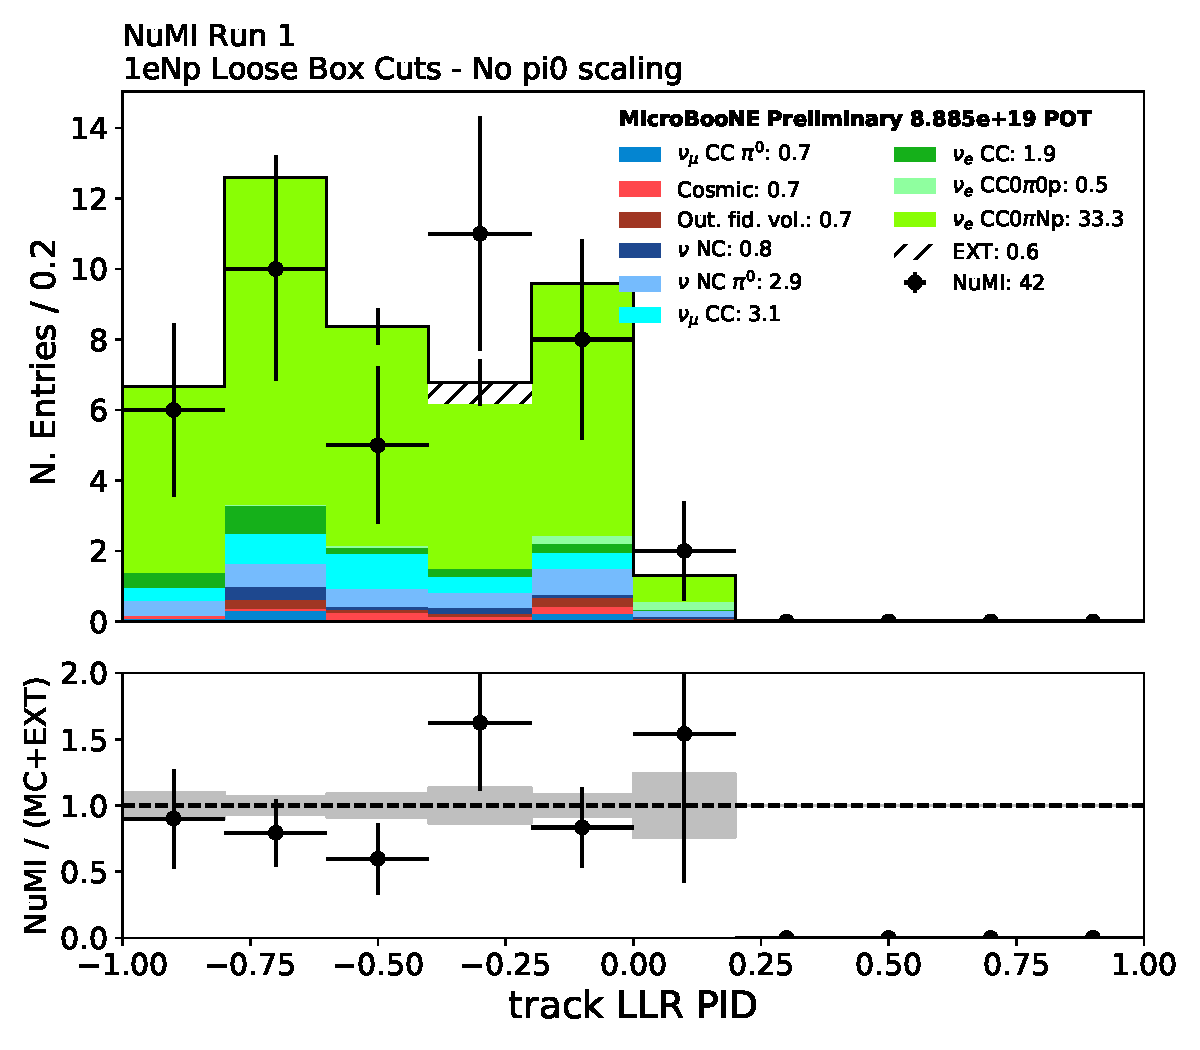
\includegraphics[width=1.0\textwidth]{Sidebands/Figures/NuMI/1eNp/trkpid.pdf}
    \caption{trkpid}
    \end{subfigure}
    \begin{subfigure}{0.3\textwidth}
    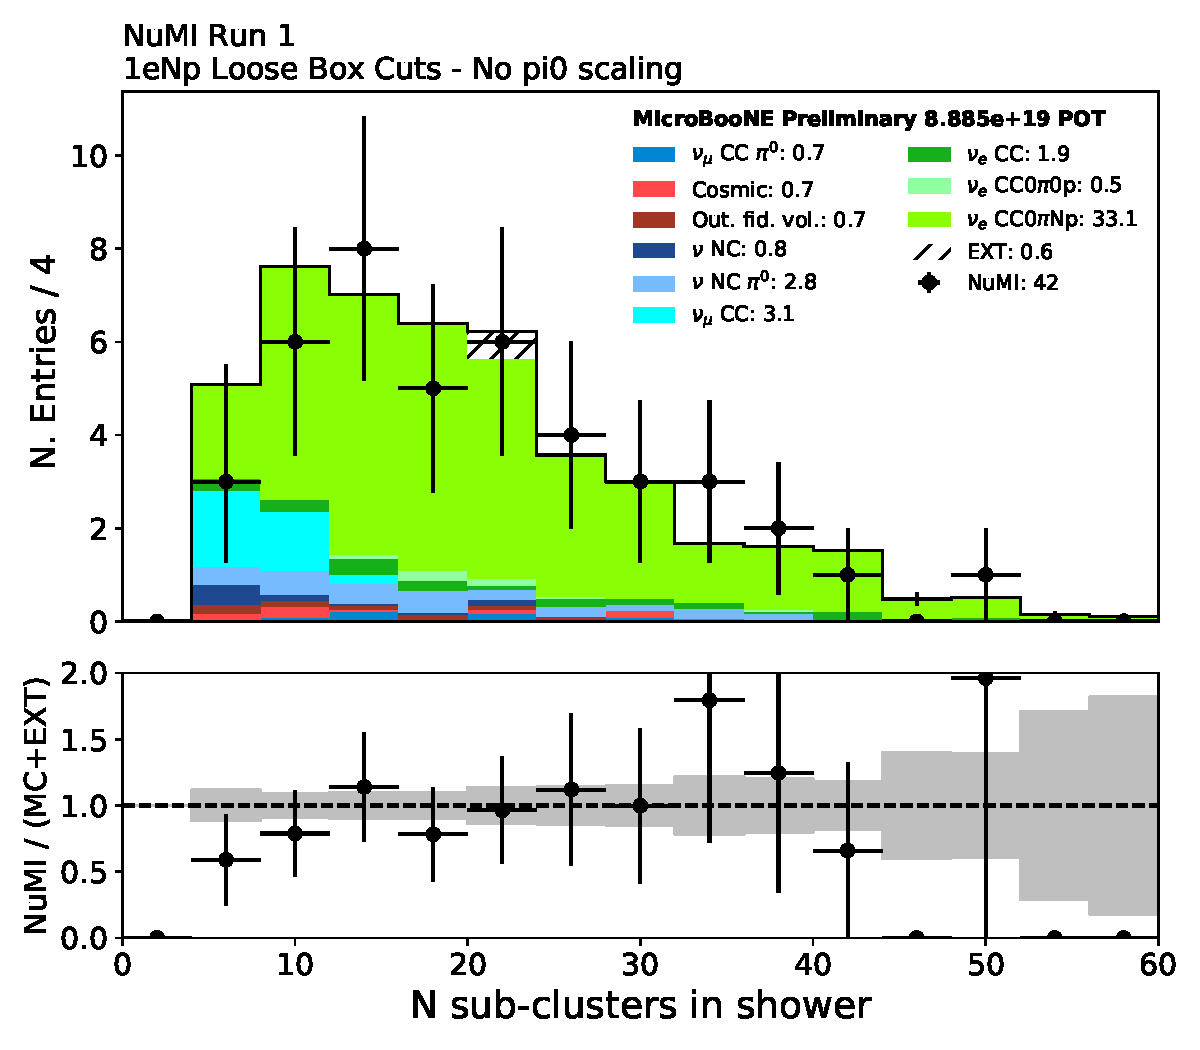
\includegraphics[width=1.0\textwidth]{Sidebands/Figures/NuMI/1eNp/subcluster.pdf}
    \caption{subcluster}
    \end{subfigure}
    \caption{} 
    \label{fig:NuMI_1eNp_2}
\end{figure}

\begin{figure}[H]
    \centering
    \begin{subfigure}{0.3\textwidth}
    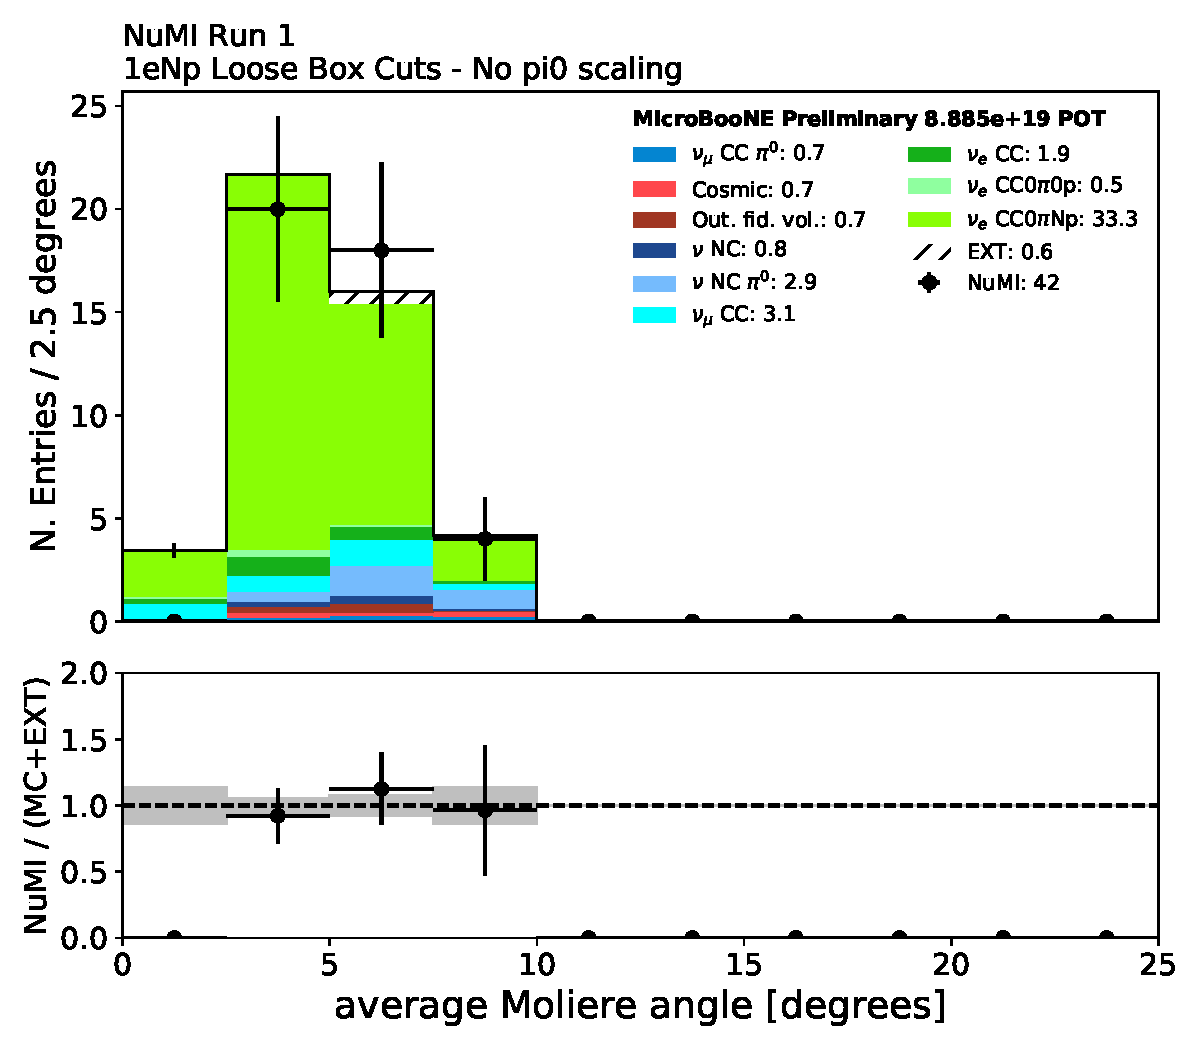
\includegraphics[width=1.0\textwidth]{Sidebands/Figures/NuMI/1eNp/shrmoliereavg.pdf}
    \caption{shrmoliereavg}
    \end{subfigure}
    \begin{subfigure}{0.3\textwidth}
    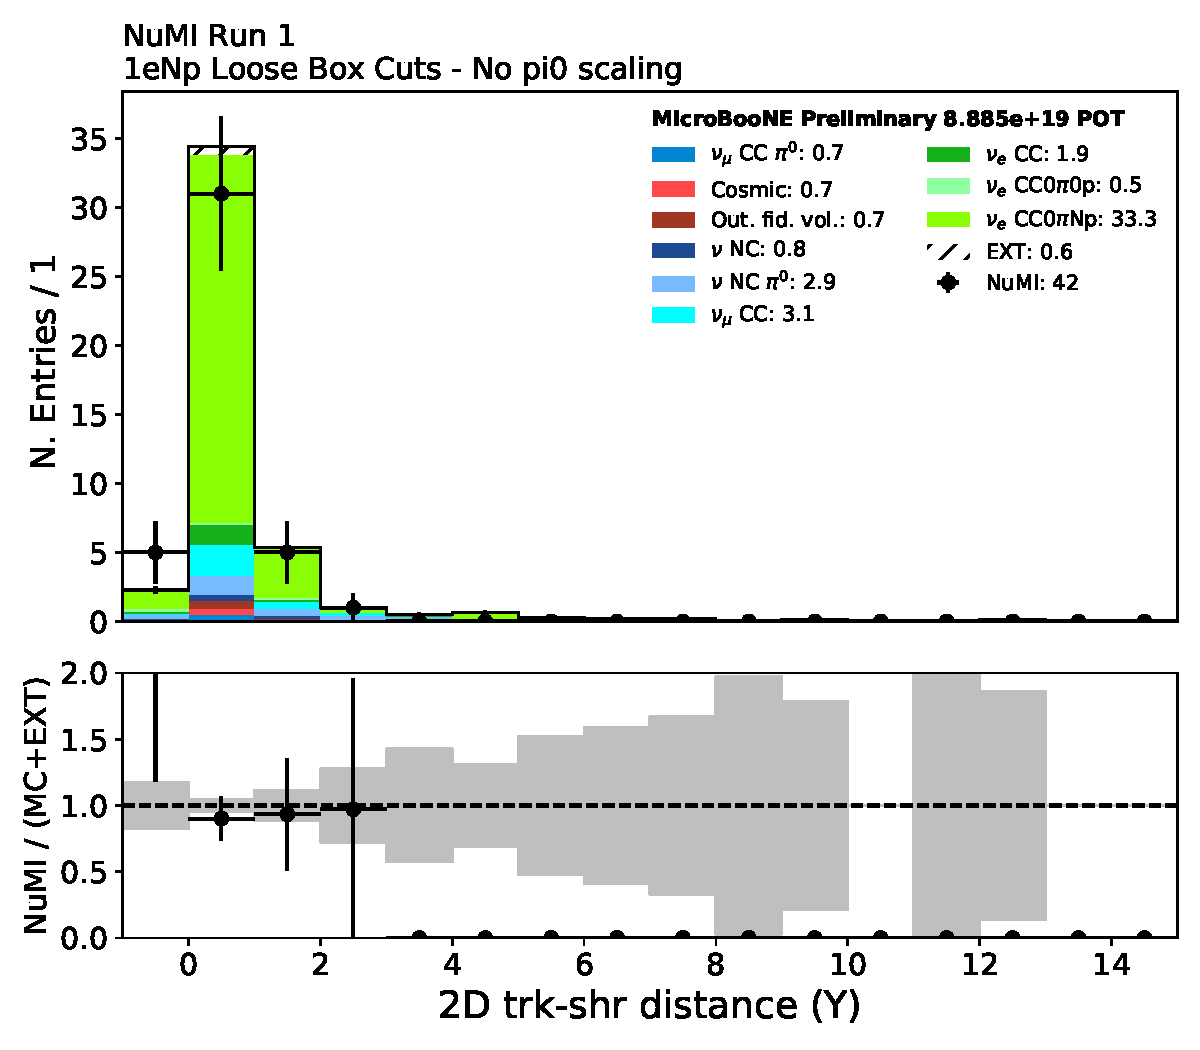
\includegraphics[width=1.0\textwidth]{Sidebands/Figures/NuMI/1eNp/trkshrhitdist2.pdf}
    \caption{tkshrhitdist2}
    \end{subfigure}
    \begin{subfigure}{0.3\textwidth}
    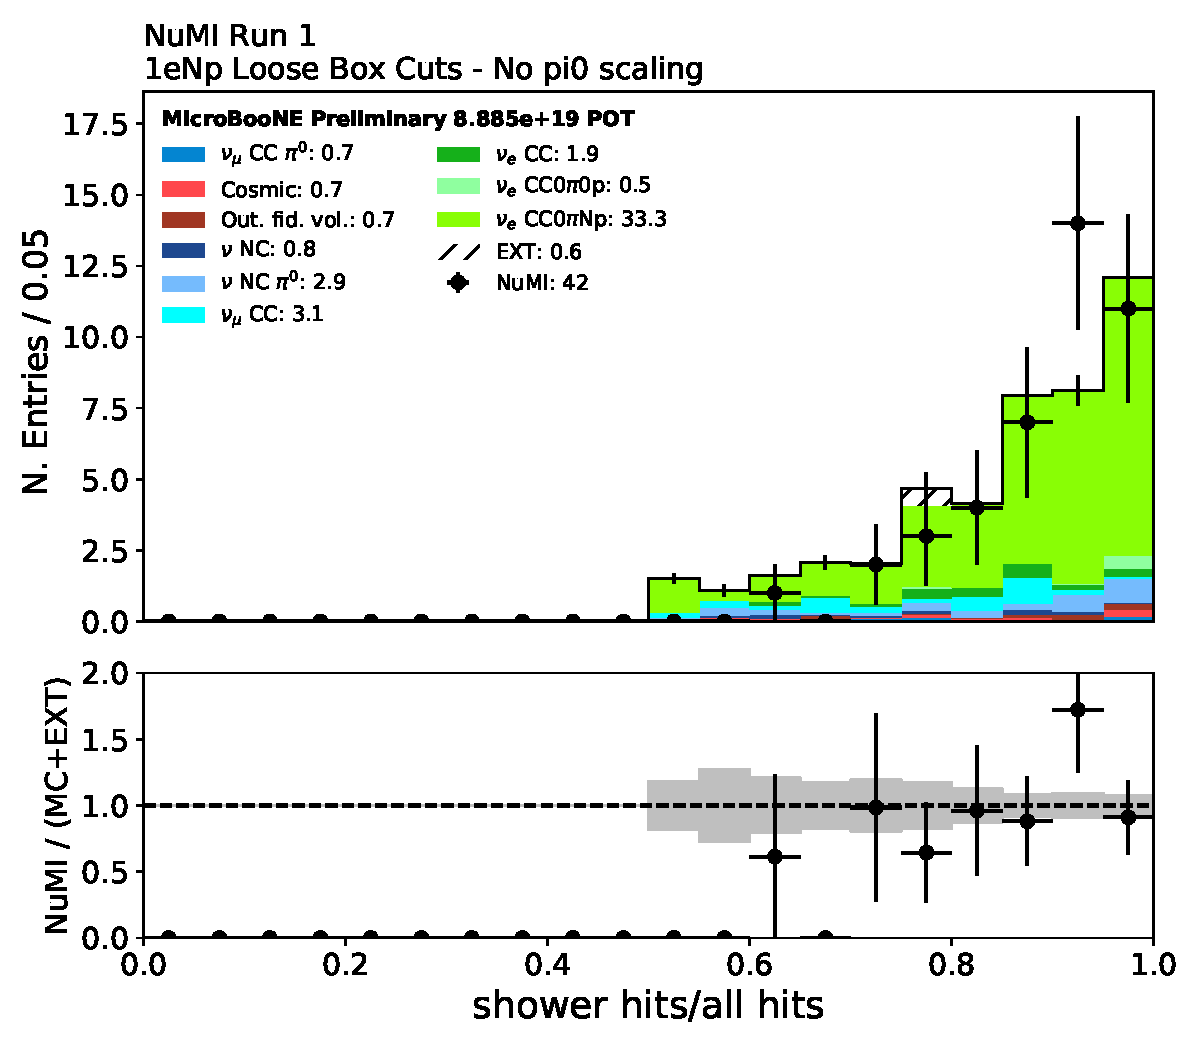
\includegraphics[width=1.0\textwidth]{Sidebands/Figures/NuMI/1eNp/hits_ratio.pdf}
    \caption{hits\_ratio}
    \end{subfigure}
    \caption{} 
    \label{fig:NuMI_1eNp_3}
\end{figure}


\begin{figure}[H]
    \centering
    \begin{subfigure}{0.3\textwidth}
    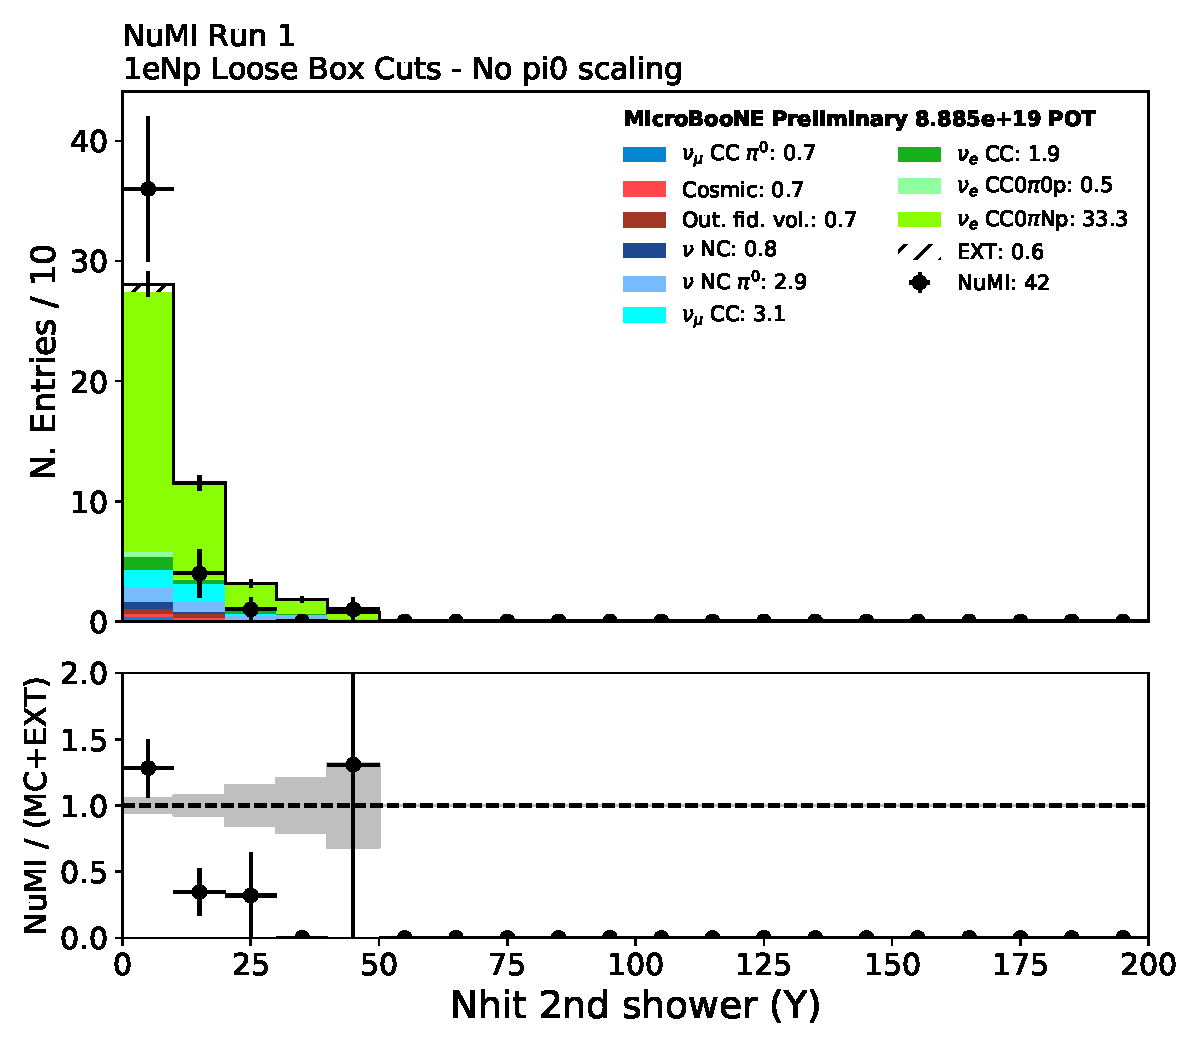
\includegraphics[width=1.0\textwidth]{Sidebands/Figures/NuMI/1eNp/secondshower_Y_nhit.pdf}
    \caption{secondshower\_Y\_nhit}
    \end{subfigure}
    \begin{subfigure}{0.3\textwidth}
    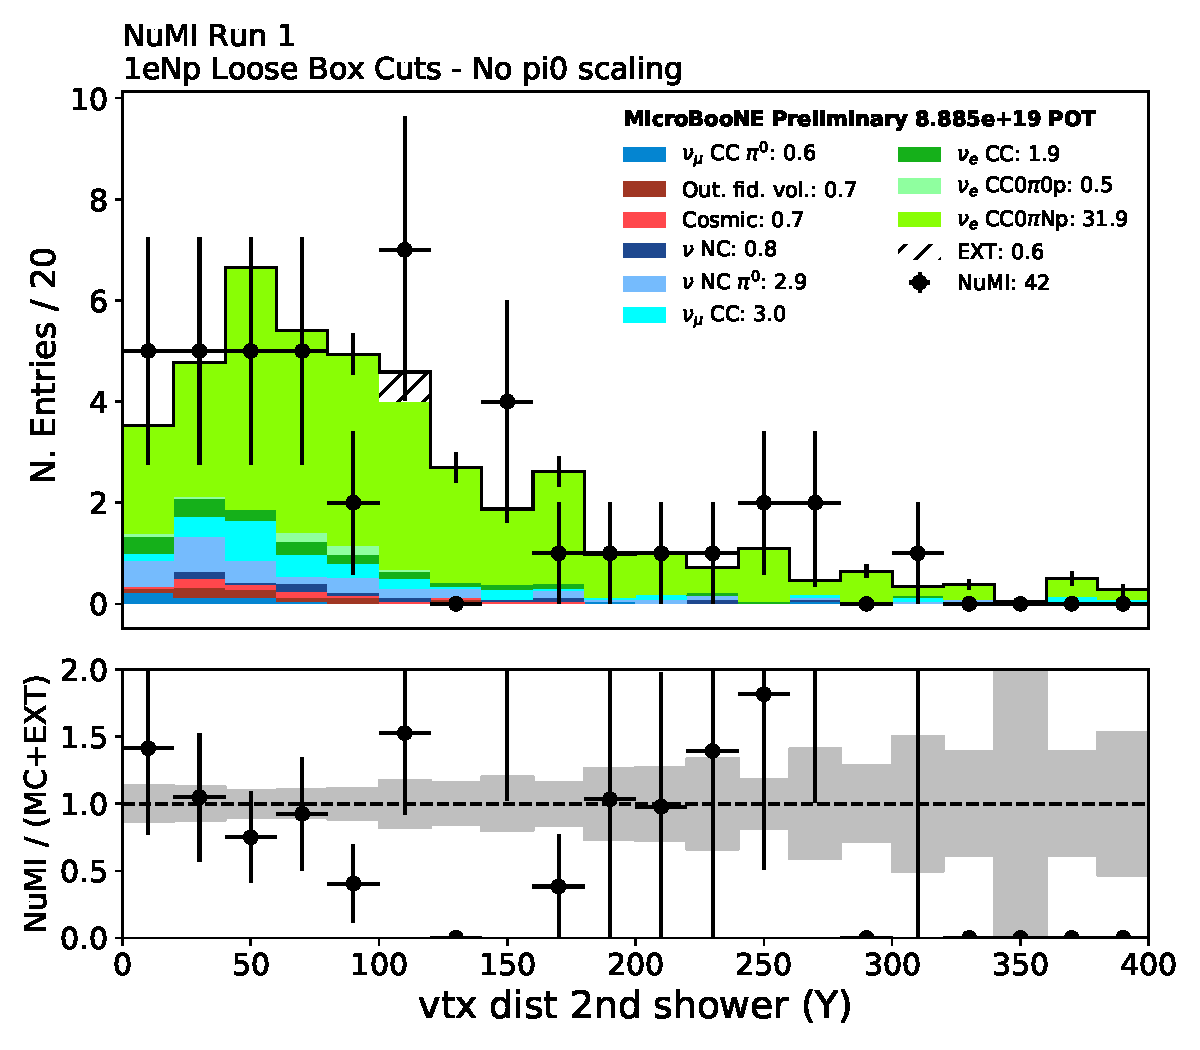
\includegraphics[width=1.0\textwidth]{Sidebands/Figures/NuMI/1eNp/secondshower_Y_vtxdist.pdf}
    \caption{secondshower\_Y\_vtxdist}
    \end{subfigure}
    \begin{subfigure}{0.3\textwidth}
    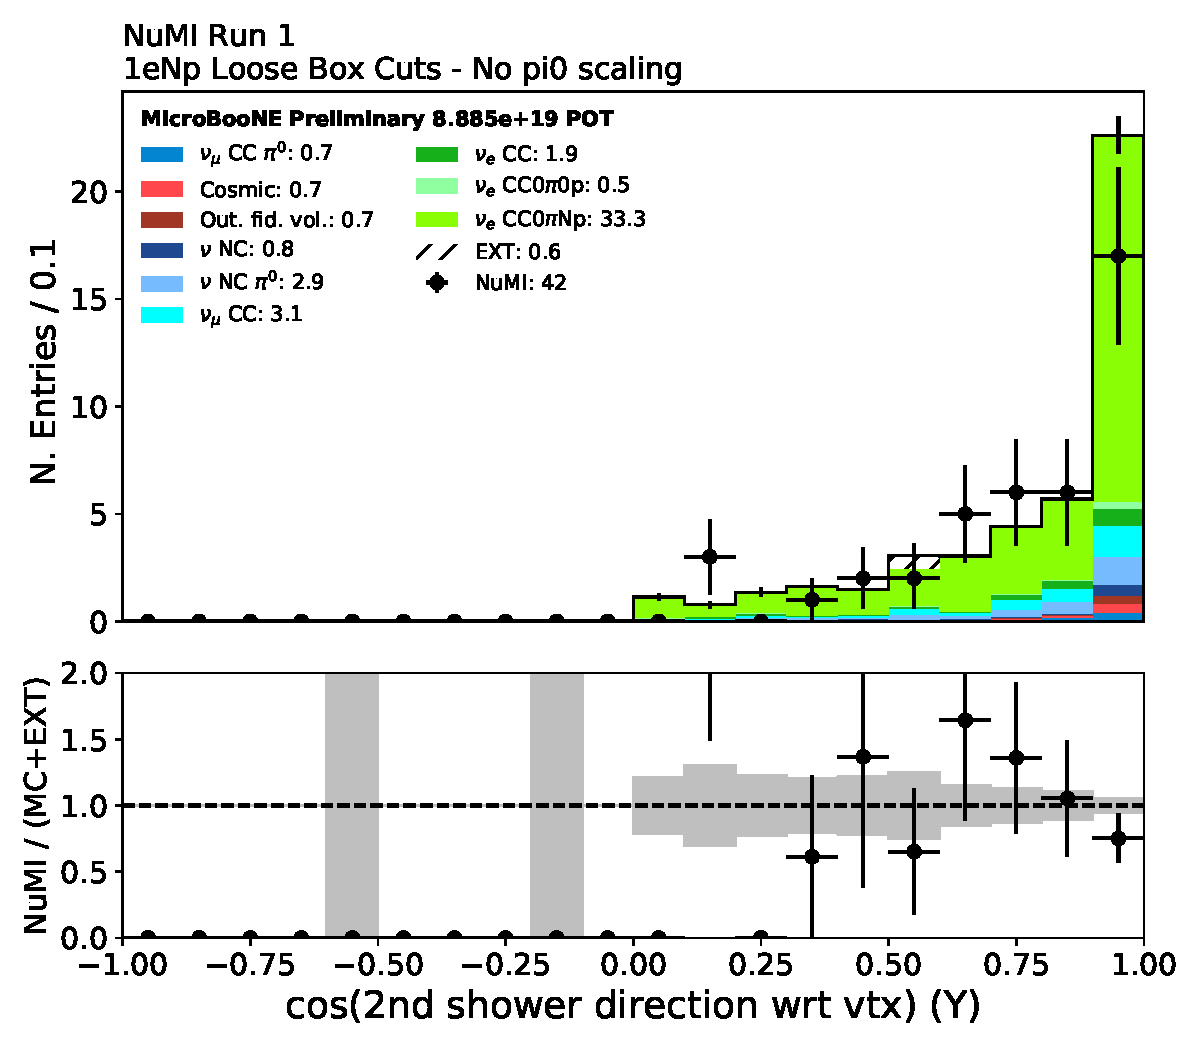
\includegraphics[width=1.0\textwidth]{Sidebands/Figures/NuMI/1eNp/secondshower_Y_dot.pdf}
    \caption{secondshower\_Y\_dot}
    \end{subfigure}
    \caption{} 
    \label{fig:NuMI_1eNp_4}
\end{figure}


\begin{figure}[H]
    \centering
    \begin{subfigure}{0.3\textwidth}
    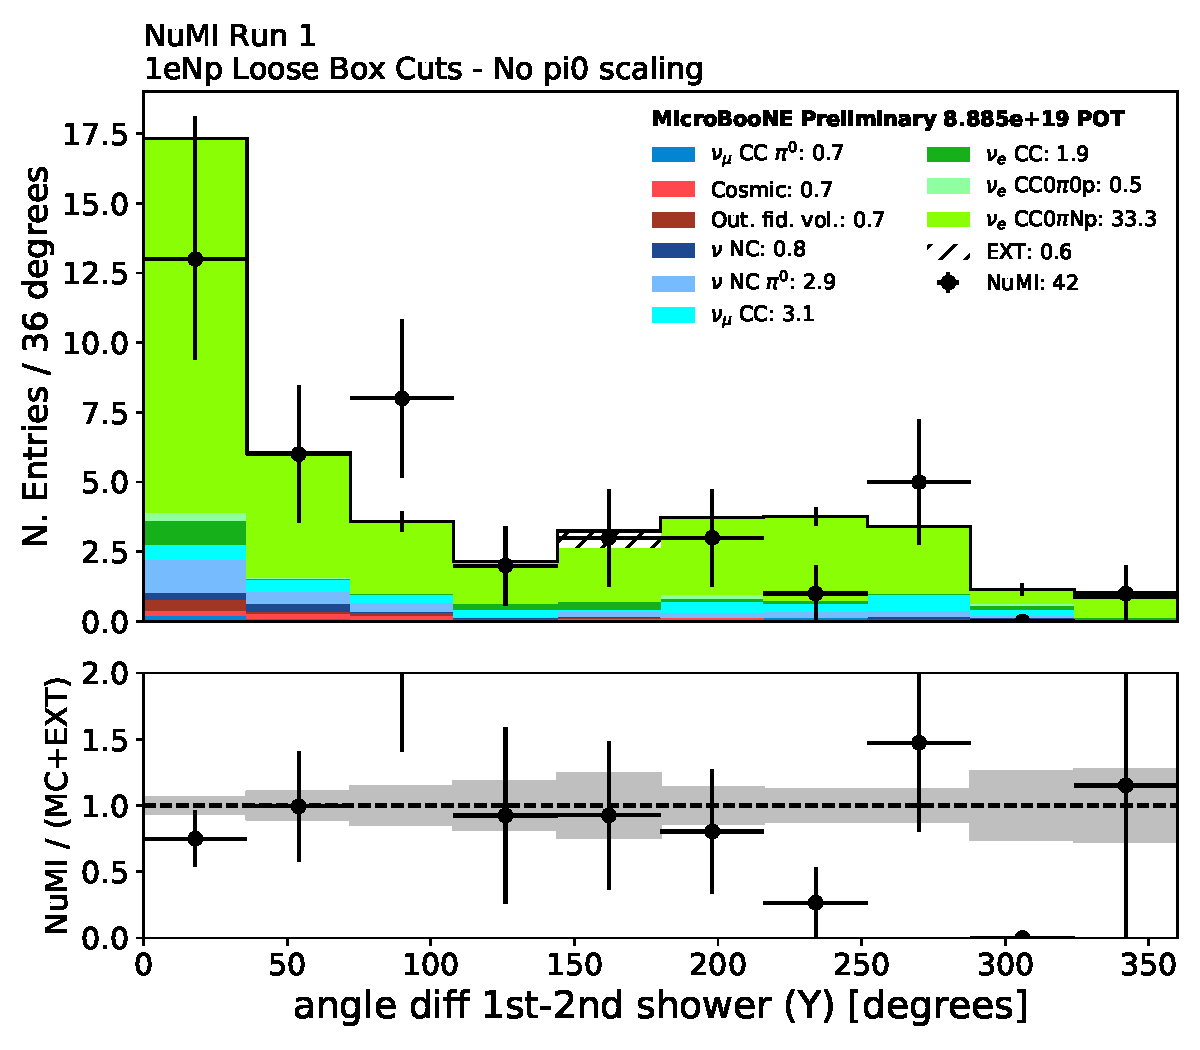
\includegraphics[width=1.0\textwidth]{Sidebands/Figures/NuMI/1eNp/anglediff_Y.pdf}
    \caption{anglediff\_Y}
    \end{subfigure}
    \begin{subfigure}{0.3\textwidth}
    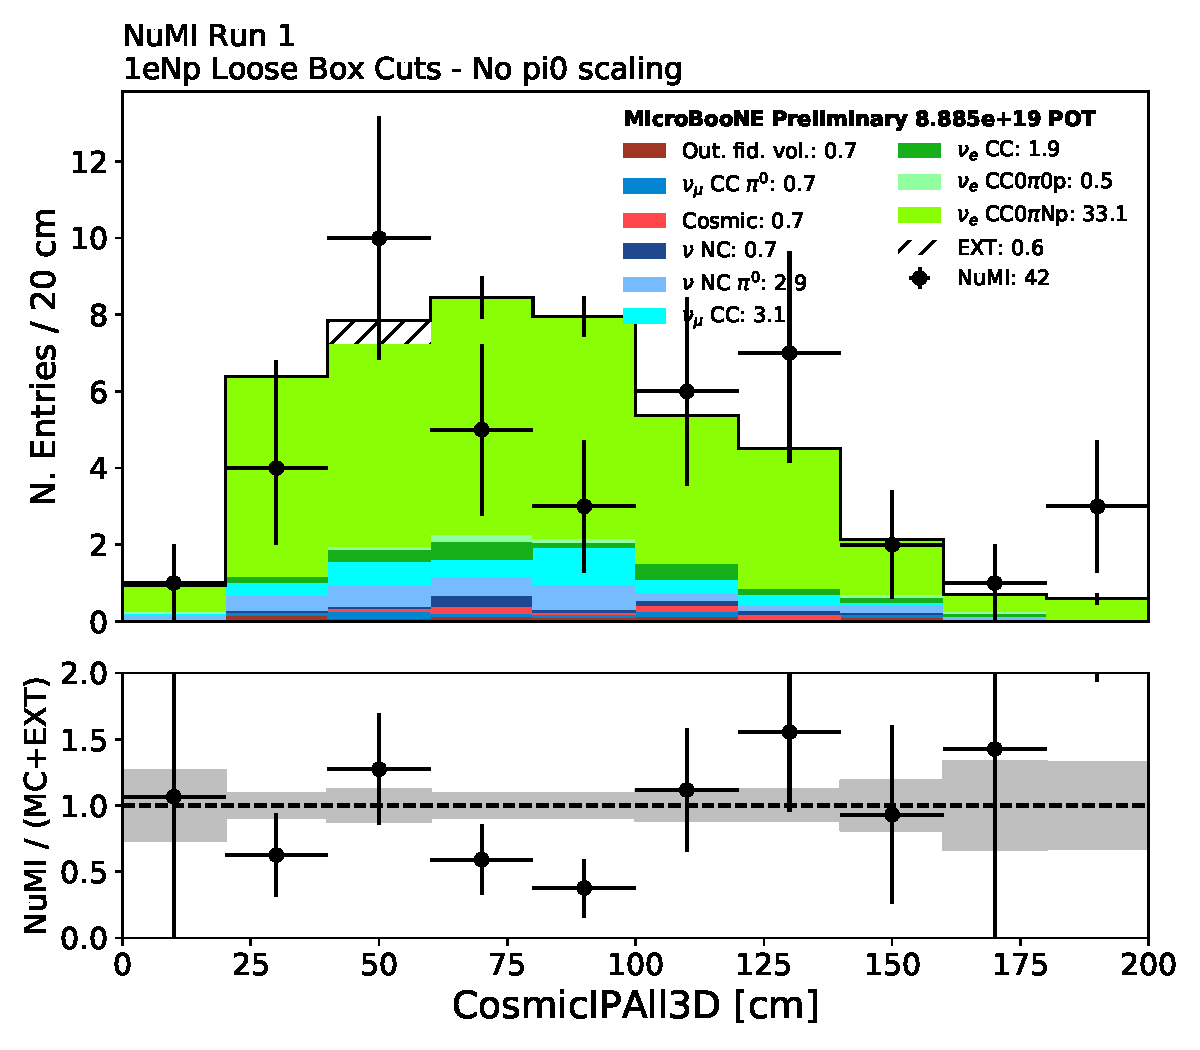
\includegraphics[width=1.0\textwidth]{Sidebands/Figures/NuMI/1eNp/CosmicIPAll3D.pdf}
    \caption{CosmicIPAll3D}
    \end{subfigure}
    \begin{subfigure}{0.3\textwidth}
    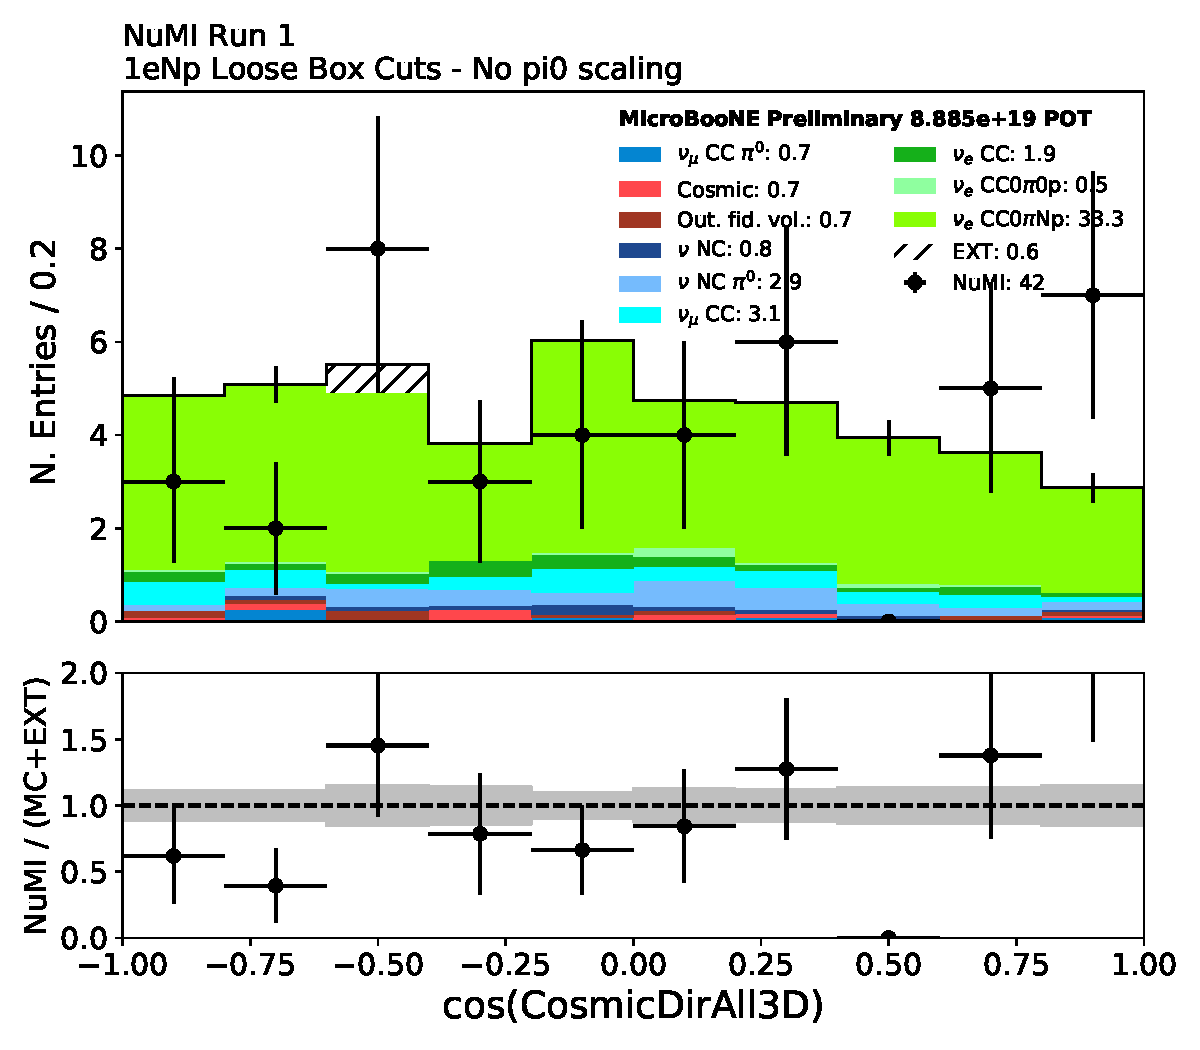
\includegraphics[width=1.0\textwidth]{Sidebands/Figures/NuMI/1eNp/CosmicDirAll3D.pdf}
    \caption{CosmidDirAll3D}
    \end{subfigure}
    \caption{} 
    \label{fig:NuMI_1eNp_5}
\end{figure}
\end{comment}



\begin{figure}[H]
    \centering
    \begin{subfigure}{0.4\textwidth}
    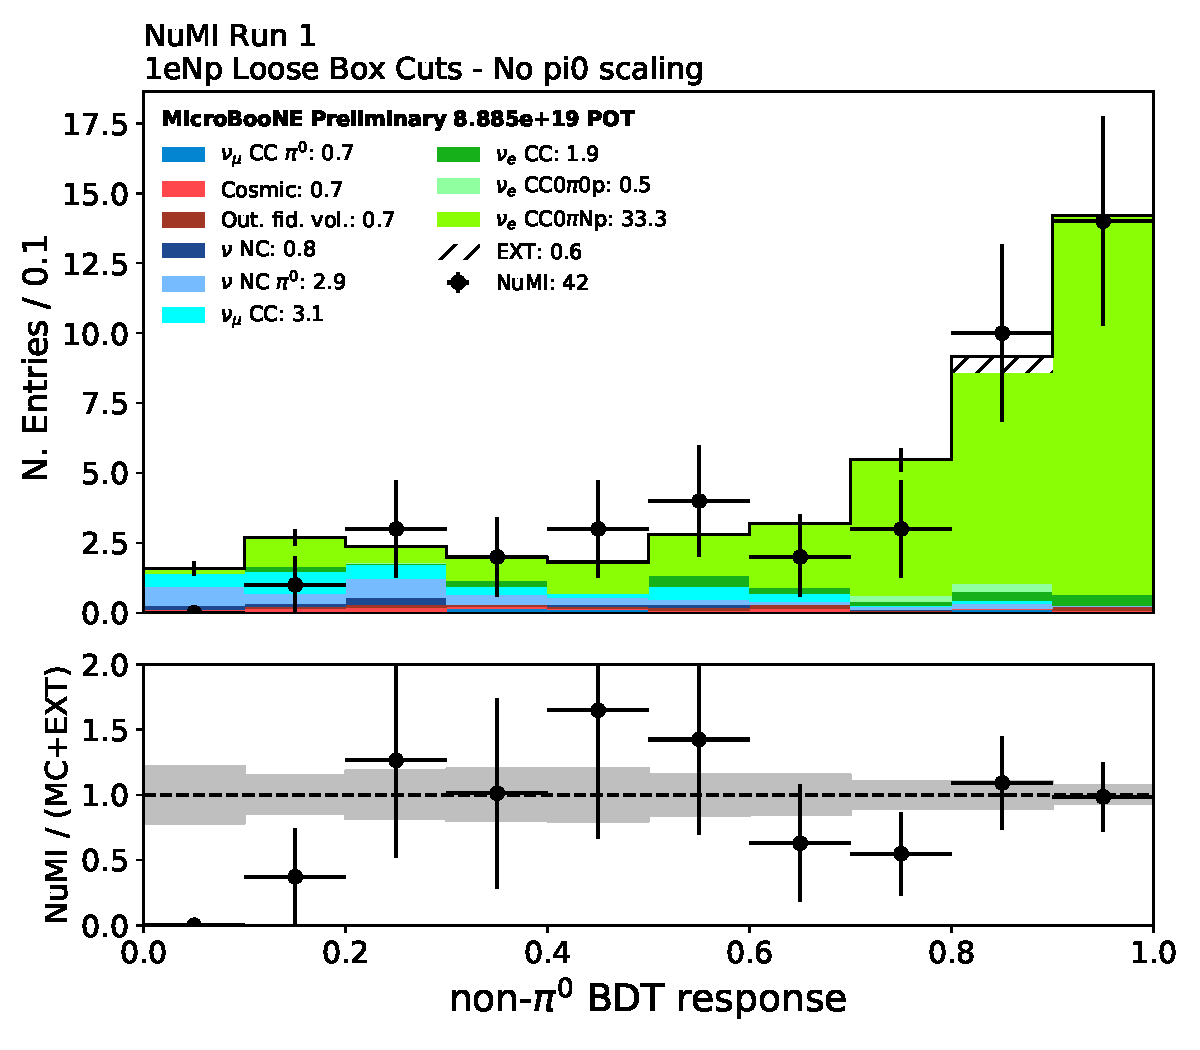
\includegraphics[width=1.0\textwidth]{Sidebands/Figures/NuMI/1eNp/nonpi0_score.pdf}
    \caption{Non $\pi^0$ BDT}
    \end{subfigure}
    \begin{subfigure}{0.4\textwidth}
    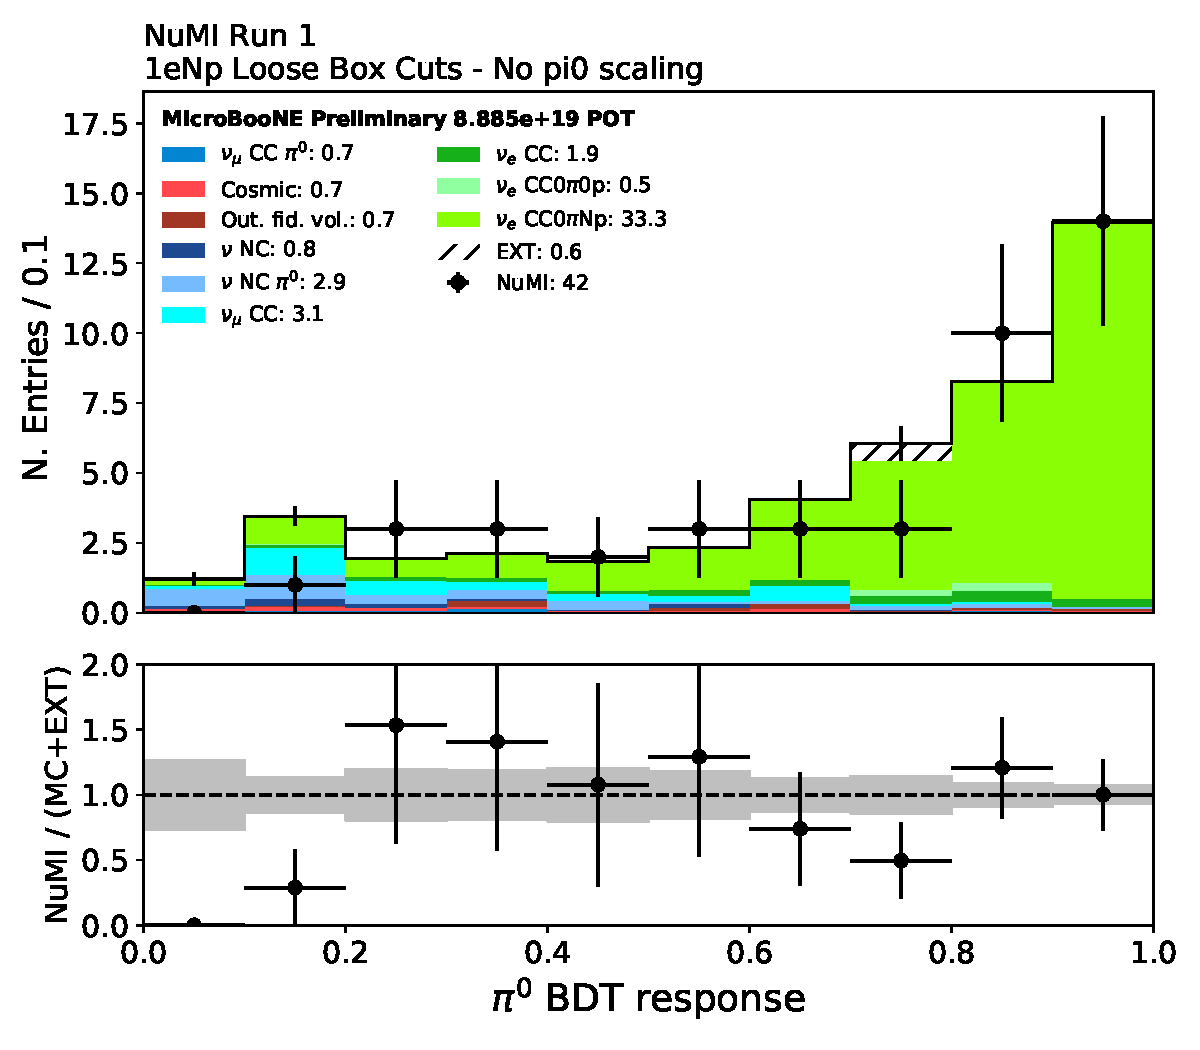
\includegraphics[width=1.0\textwidth]{Sidebands/Figures/NuMI/1eNp/pi0_score.pdf}
    \caption{$\pi^0$ BDT}
    \end{subfigure}
    \caption{BDT responses after \npsel Loose selection on NuMI data.} 
    \label{fig:NuMI_1eNp_7}
\end{figure}



Figures~\ref{fig:NuMI_1eNp_9} and~\ref{fig:NuMI_1eNp_10} show select kinematics distributions for selected \npsel events.

\begin{figure}[H]
    \centering
    \begin{subfigure}{0.3\textwidth}
    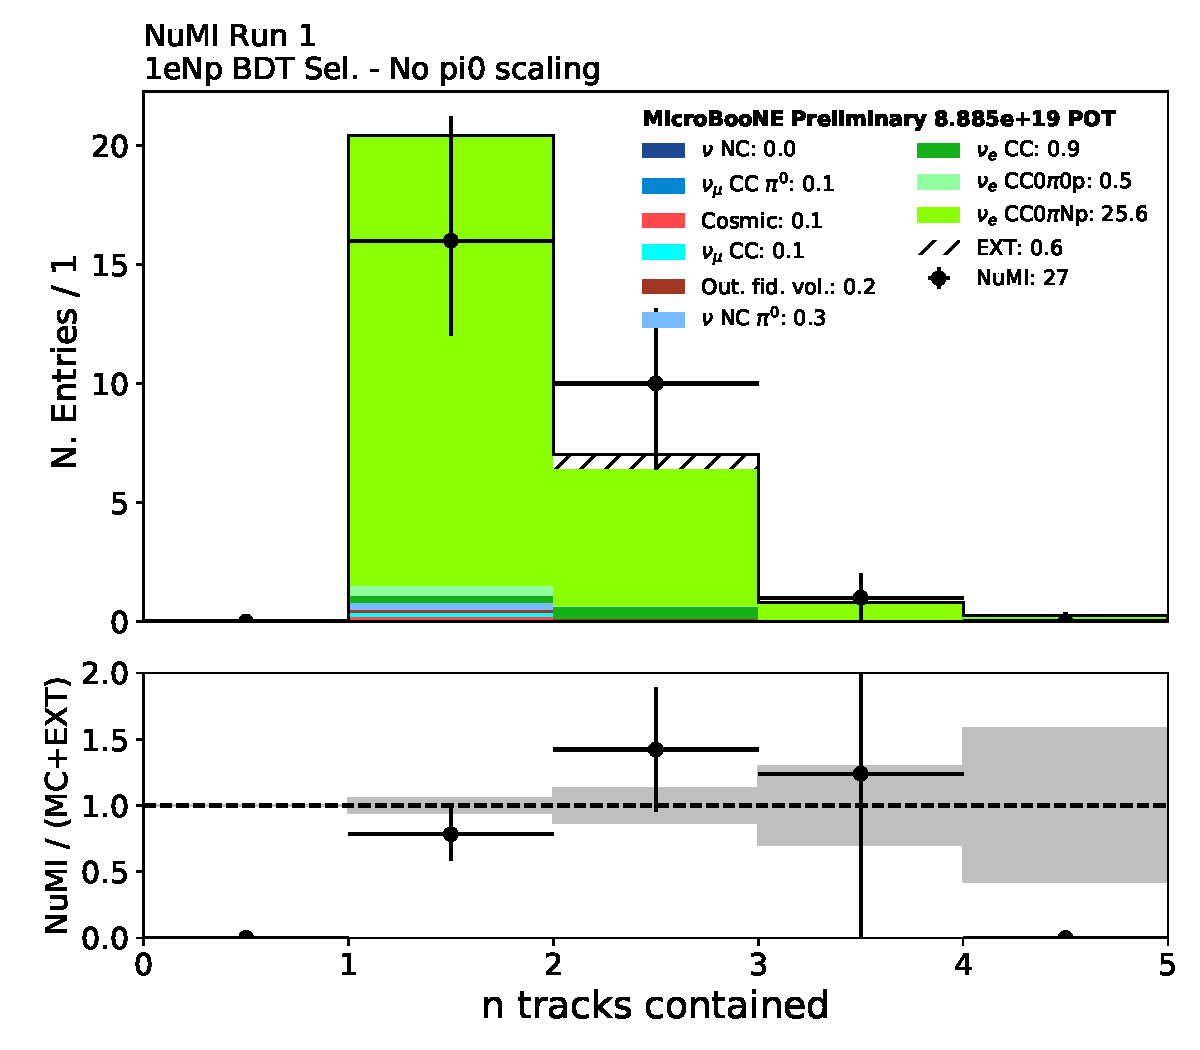
\includegraphics[width=1.0\textwidth]{Sidebands/Figures/NuMI/1eNp/BDTSel/n_tracks_contained.pdf}
    \caption{}
    \end{subfigure}
    \begin{subfigure}{0.3\textwidth}
    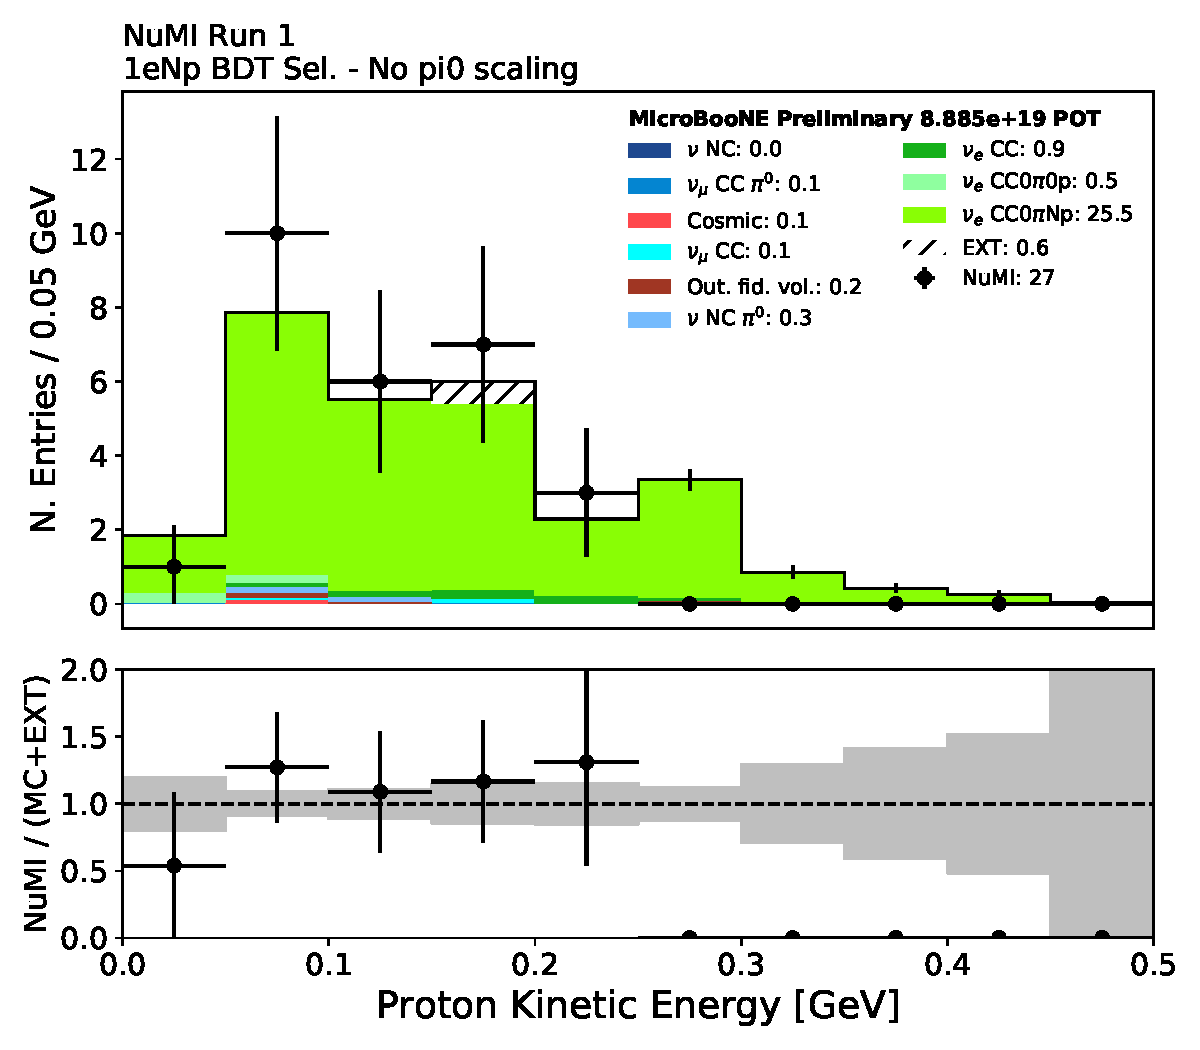
\includegraphics[width=1.0\textwidth]{Sidebands/Figures/NuMI/1eNp/BDTSel/protonenergy.pdf}
    \caption{}
    \end{subfigure}
    \begin{subfigure}{0.3\textwidth}
    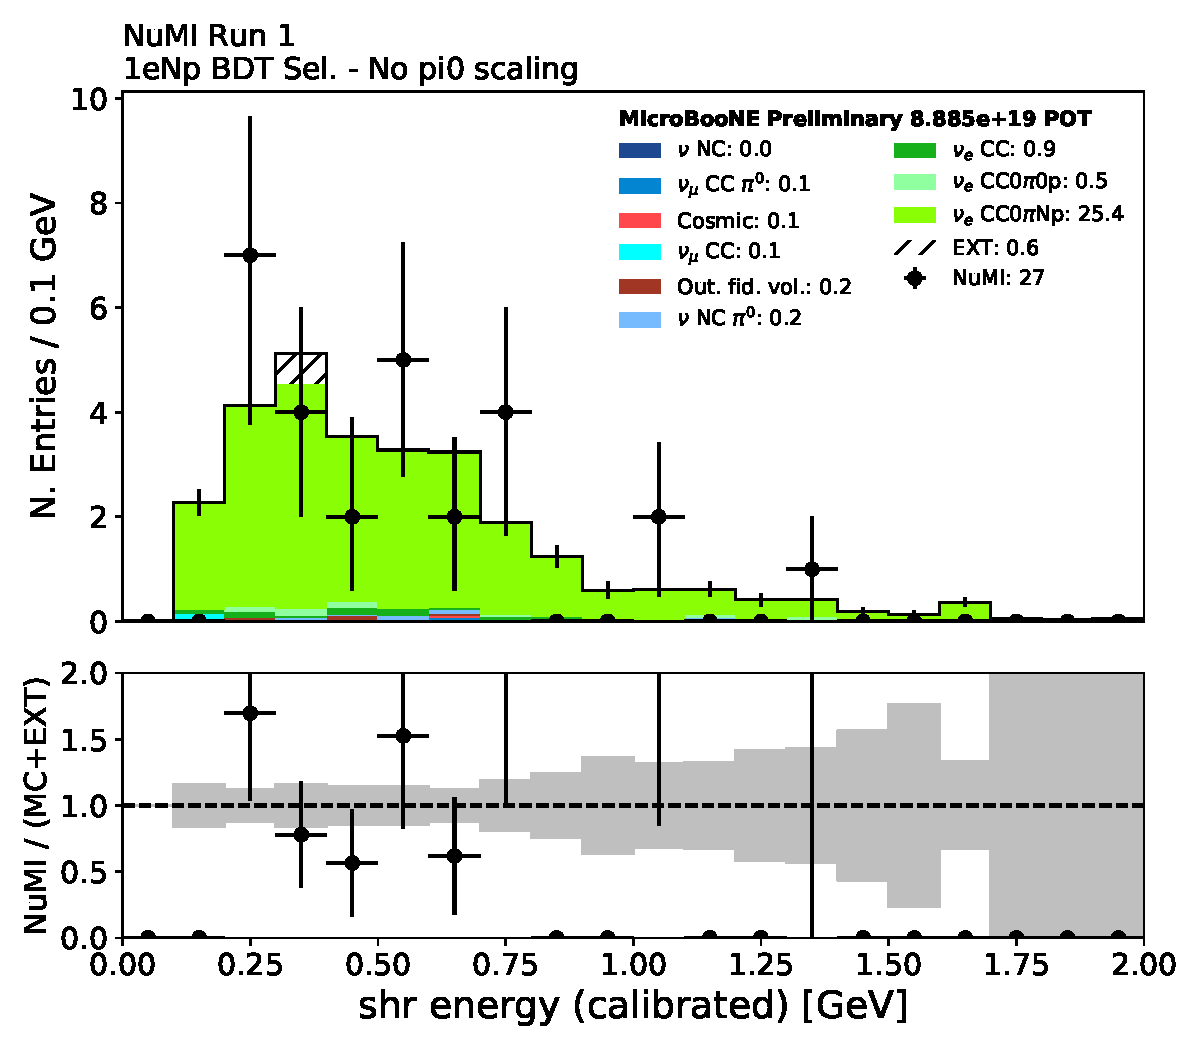
\includegraphics[width=1.0\textwidth]{Sidebands/Figures/NuMI/1eNp/BDTSel/shr_energy_tot_cali.pdf}
    \caption{}
    \end{subfigure}
    \caption{Select kinematic variables after \npsel BDT selection on NuMI data.} 
    \label{fig:NuMI_1eNp_9}
\end{figure}

\begin{figure}[H]
    \centering
    \begin{subfigure}{0.3\textwidth}
    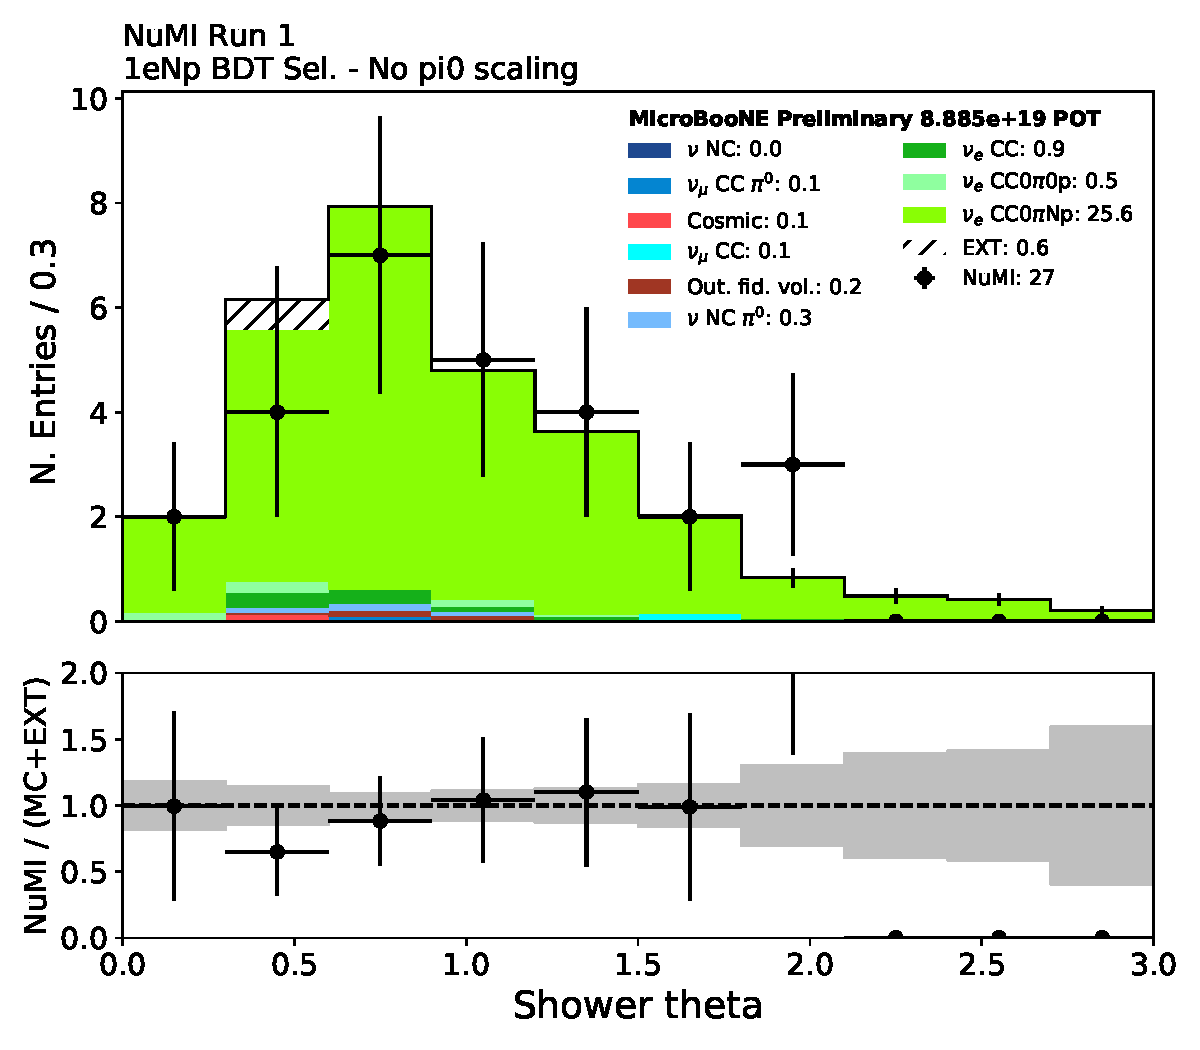
\includegraphics[width=1.0\textwidth]{Sidebands/Figures/NuMI/1eNp/BDTSel/shr_theta.pdf}
    \caption{}
    \end{subfigure}
    \begin{subfigure}{0.3\textwidth}
    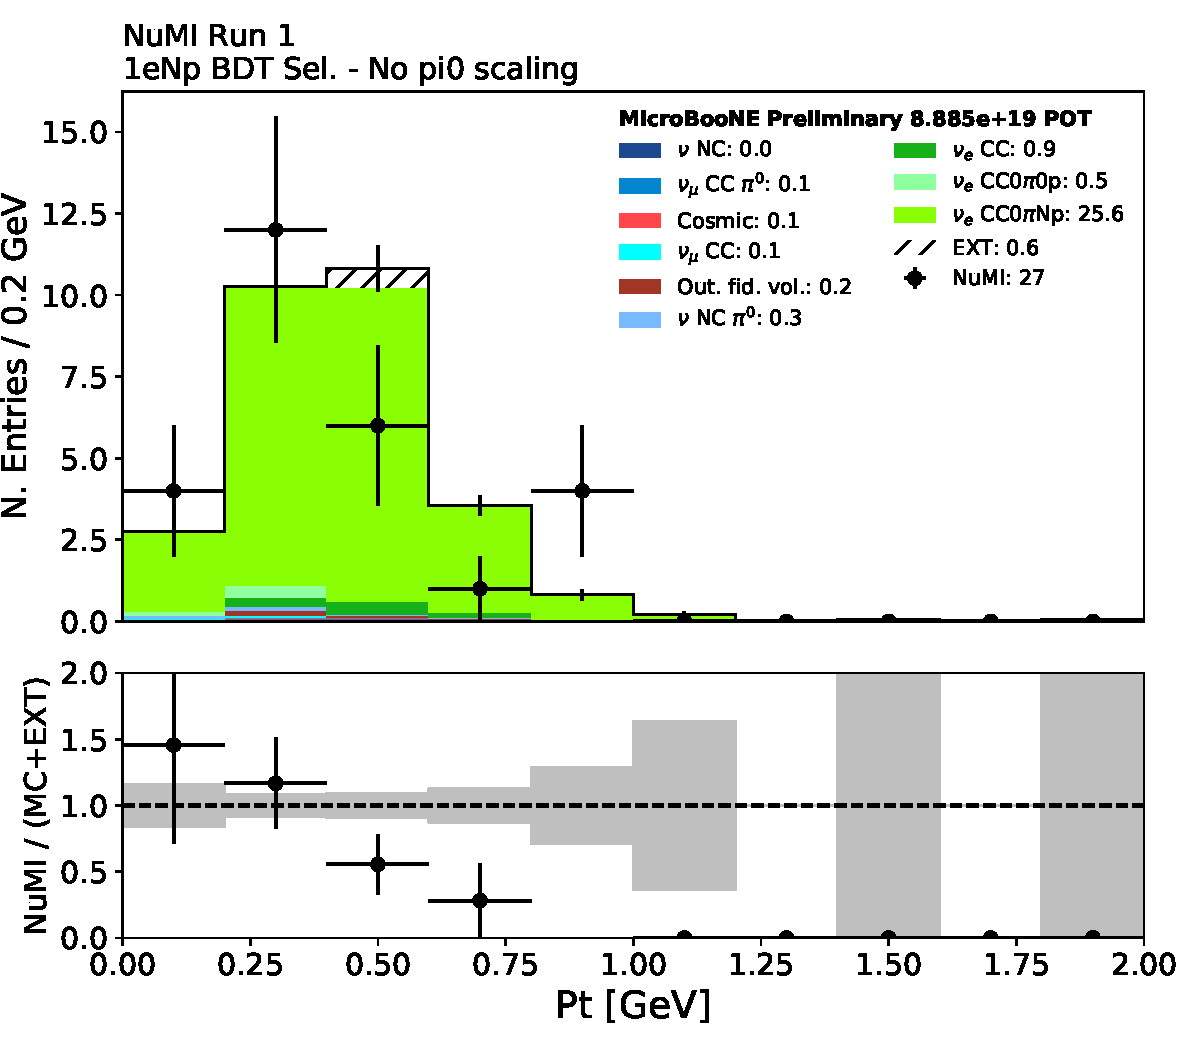
\includegraphics[width=1.0\textwidth]{Sidebands/Figures/NuMI/1eNp/BDTSel/pt.pdf}
    \caption{}
    \end{subfigure}
    \begin{subfigure}{0.3\textwidth}
    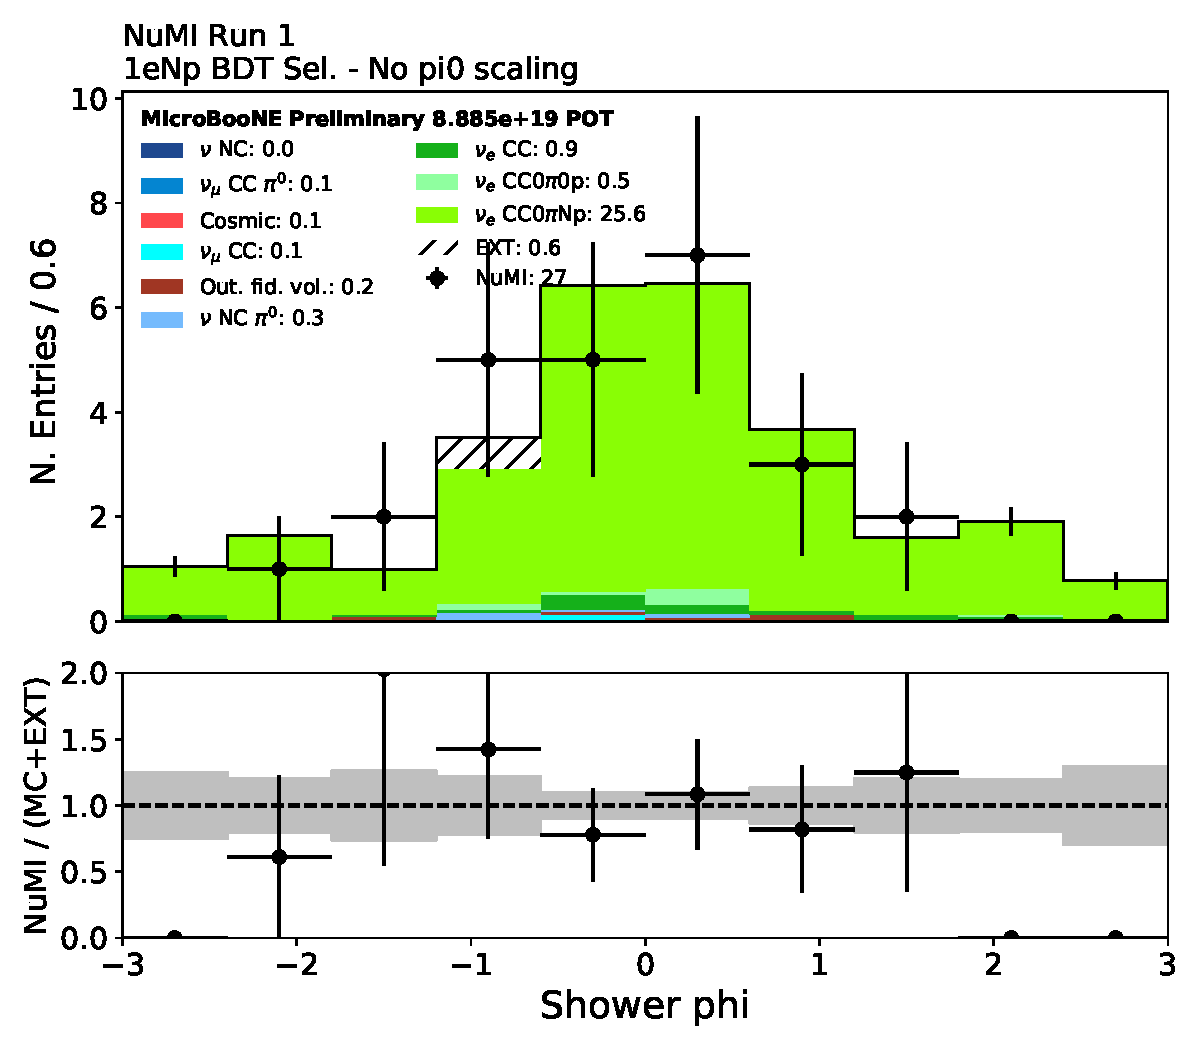
\includegraphics[width=1.0\textwidth]{Sidebands/Figures/NuMI/1eNp/BDTSel/shr_phi.pdf}
    \caption{}
    \end{subfigure}
    \caption{Select kinematic variables after \npsel BDT selection on NuMI data.} 
    \label{fig:NuMI_1eNp_10}
\end{figure}

Figure~\ref{fig:Numi1enpEvd} shows the 6 events with energy lower than 500 MeV identified in the NuMI dataset by the \npsel final selection.


\begin{figure}[H]
    \begin{center}
    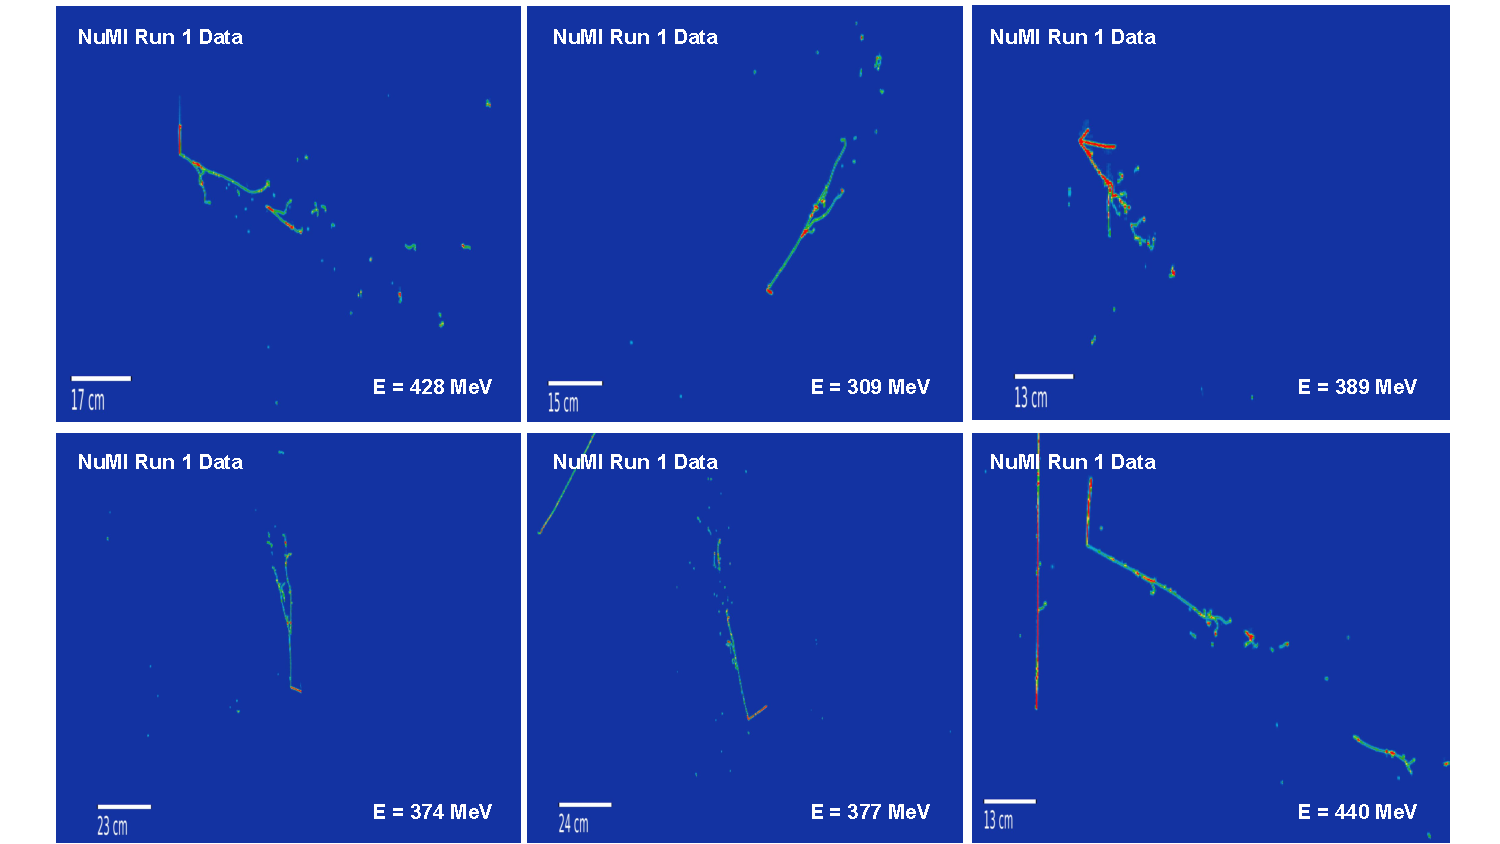
\includegraphics[width=\textwidth]{Sidebands/Figures/NuMI/1eNp/BDTSel/Evds.pdf}
    \caption{Event displays for low energy events selected by the \npsel BDT selection on NuMI data.}
    \label{fig:Numi1enpEvd}
    \end{center}
\end{figure}

\subsubsection{NuMI $\pi^0$ Sideband}
The NuMI dataset allows for an independent study of data events rich in $\pi^0$s. As illustrated in section \cref{sec:sideband:pi0}, such events have shown a significant tension with MC expectations for the BNB dataset. Applying the identical selection described in \cref{tab:pi0sideband} to the NuMI dataset results in an analogous deficit of data events compared to the MC predictions, as exemplified by  \cref{fig:pi0NuMI:noscale} for the $\pi^0$ mass distribution.  After the application of the $\pi^0$ tune obtained from the BNB data, the Data-MC agreement significantly improves in NuMI. As for the BNB case, the best agreement for this selection is obtained when a flat scaling is applied to MC events containing a $\pi^0$ (see \cref{fig:pi0NuMI:flatscale}). An improvement is also obtained when the tune is applied as a function of the $\pi^0$ energy (see \cref{fig:pi0NuMI:Escale}). 
Since the NuMI and BNB predictions for the fluxes at MicroBooNE are completely independent, such a similar data deficit of $\pi^0$ enriched events in x both the samples suggests that the cause of this Data-MC tension is likely a cross section mis-modeling. As for the previous NuMI sideband, we are expecting sizable flux and cross section systematics, which might cover the remaining discrepancies and are not currently considered.  A deeper explorations of $\pi^0$s in NuMI is documented in Ref.~\cite{bib:NuMIPi0}.

\begin{figure}[H] 
\begin{center}
    \begin{subfigure}[b]{0.29\textwidth}
    \centering
    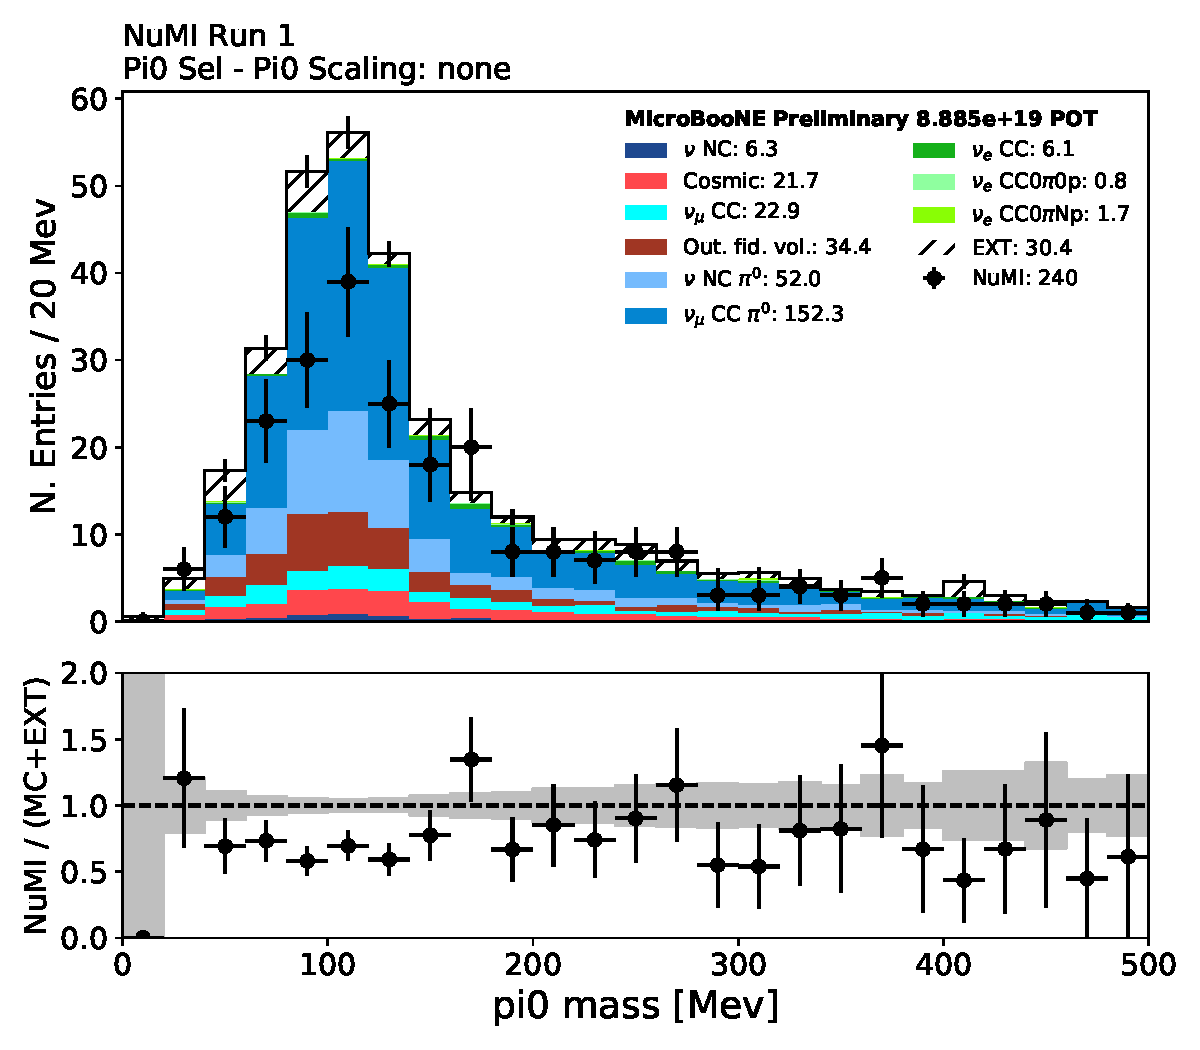
\includegraphics[width=1.00\textwidth]{Sidebands/Figures/NuMI/Pi0/pi0_mass_Y_NoScale.pdf}
    \caption{\label{fig:pi0NuMI:noscale} No scaling}
    \end{subfigure}
    \begin{subfigure}[b]{0.29\textwidth}
    \centering
    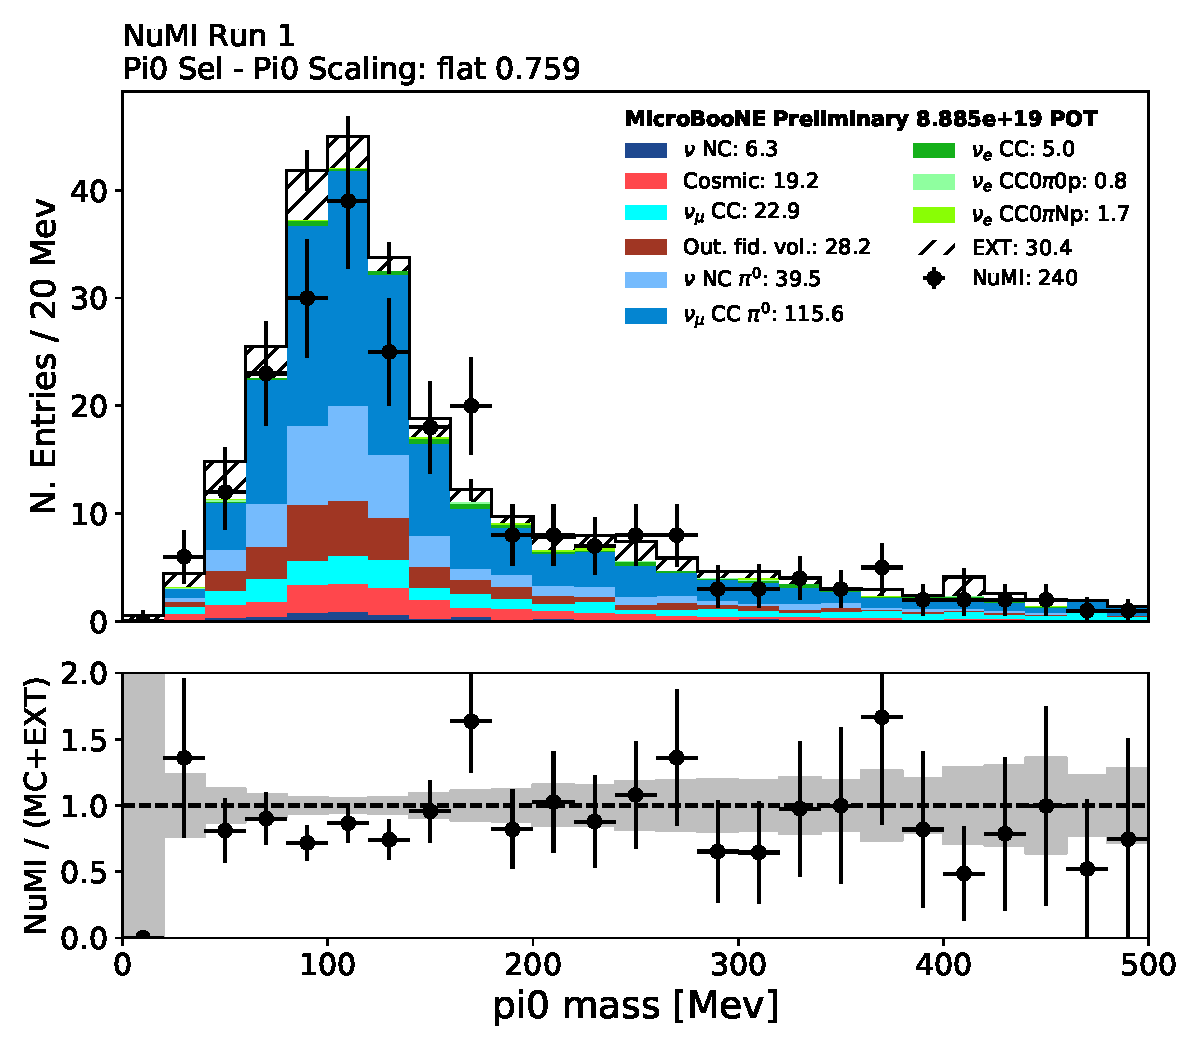
\includegraphics[width=1.00\textwidth]{Sidebands/Figures/NuMI/Pi0/pi0_mass_Y_FlatScale.pdf}
    \caption{\label{fig:pi0NuMI:flatscale} After flat scaling.}
    \end{subfigure}
    \begin{subfigure}[b]{0.29\textwidth}
    \centering
    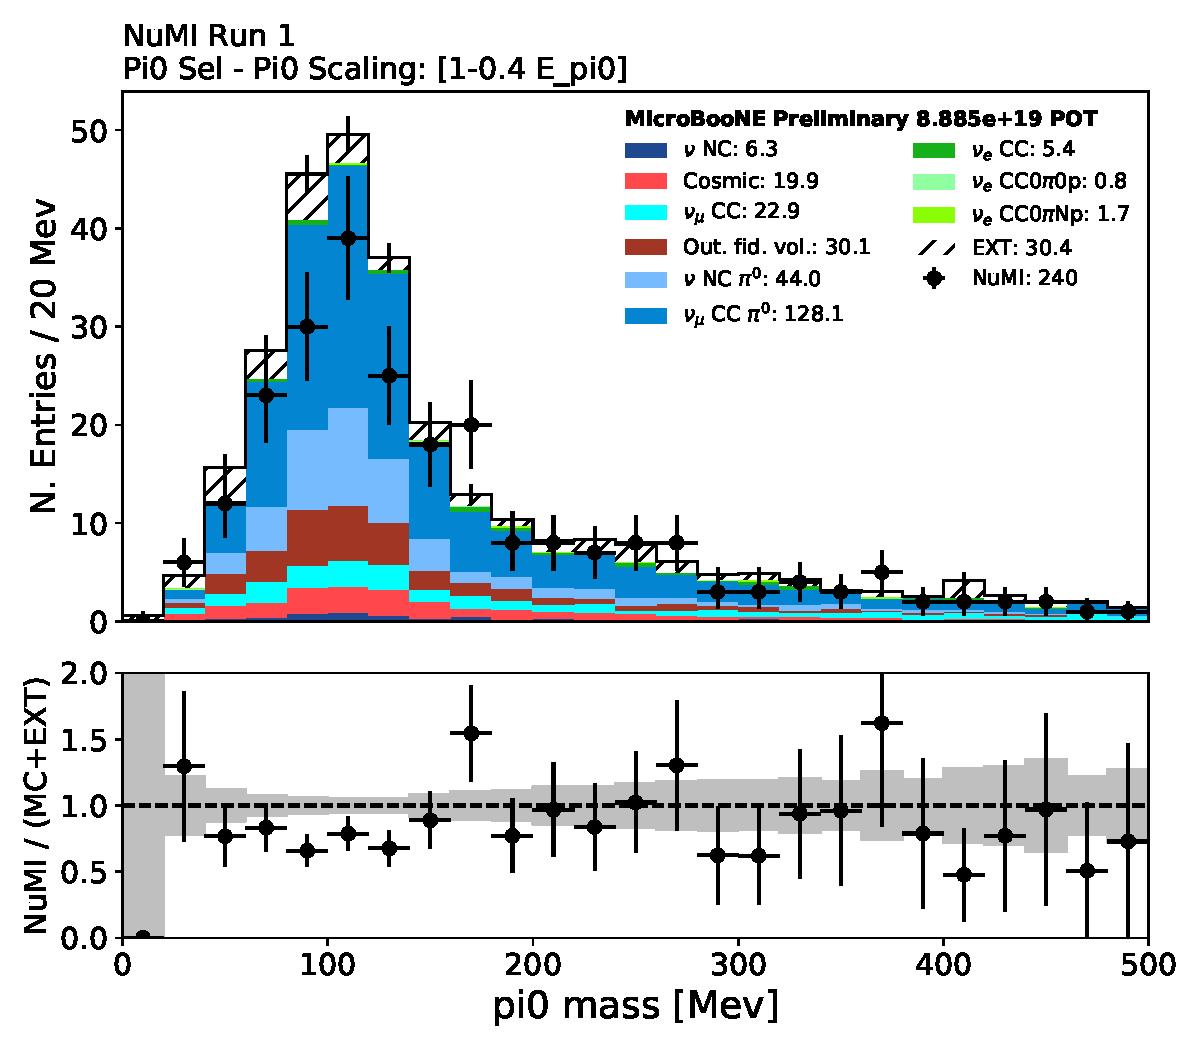
\includegraphics[width=1.00\textwidth]{Sidebands/Figures/NuMI/Pi0/pi0_mass_Y_ScaleE.pdf}
    \caption{\label{fig:pi0NuMI:Escale} After energy dependent scaling}
    \end{subfigure}
\caption{\label{fig:pi0NuMI} $\pi^0$ mass in NuMI $\pi^0$ enriched sample. }
\end{center}
\end{figure}







